\chapter{Risultati sperimentali}
\label{chap:risultati}

\section{Hand Detection}
\label{sec:risultati_detection}

\begin{table}[H]
\centering
\caption{Risultati del modello di hand detection sui tre split. La mAP è calcolata su soglie di IoU (Sez.~\ref{sec:iou_map}).}
\label{tab:risultati_bbox}
\smallskip
\begin{tabular}{lccc}
\toprule
Split & mAP@[.5:.95] & mAP@.50 & mAP@.75 \\
\midrule
Train & 0.9159 & 0.9888 & 0.9866 \\
Val   & 0.8856 & 0.9842 & 0.9443 \\
Test  & 0.9219 & 0.9791 & 0.9791 \\
\bottomrule
\end{tabular}
\end{table}

I risultati sono consistenti tra i tre split, senza segnali di
overfitting. Il paper BoNet~\cite{escobar2019bonet} riporta
mAP@[.5:.95] = 90.1\% sul validation set con l'intero training set; il
valore ottenuto (88.56\%) è comparabile
nonostante l'addestramento su un sottoinsieme di sole 250 immagini.

\begin{figure}[H]
\centering
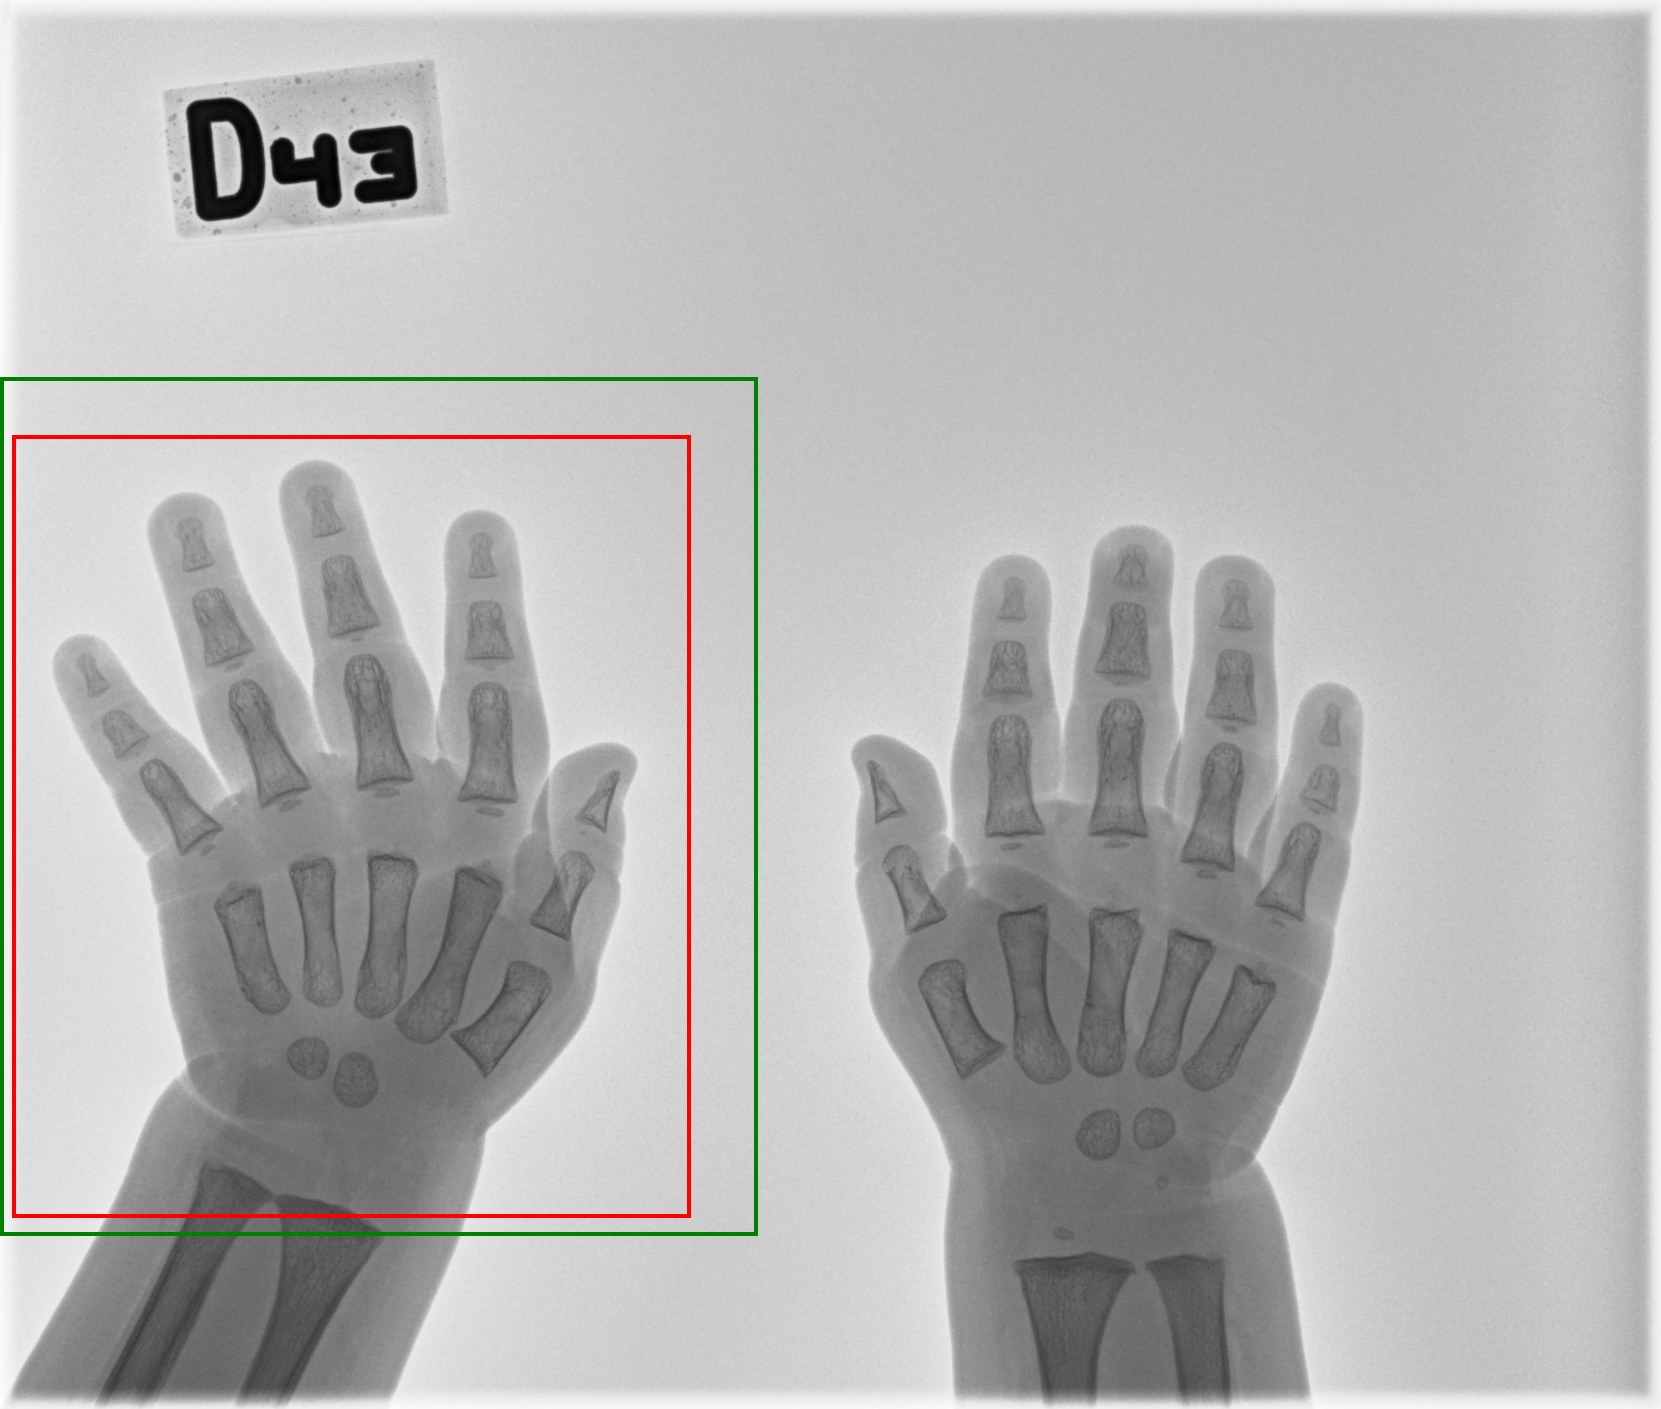
\includegraphics[width=0.32\textwidth]{figure/esempiobbox1.jpg}\hfill
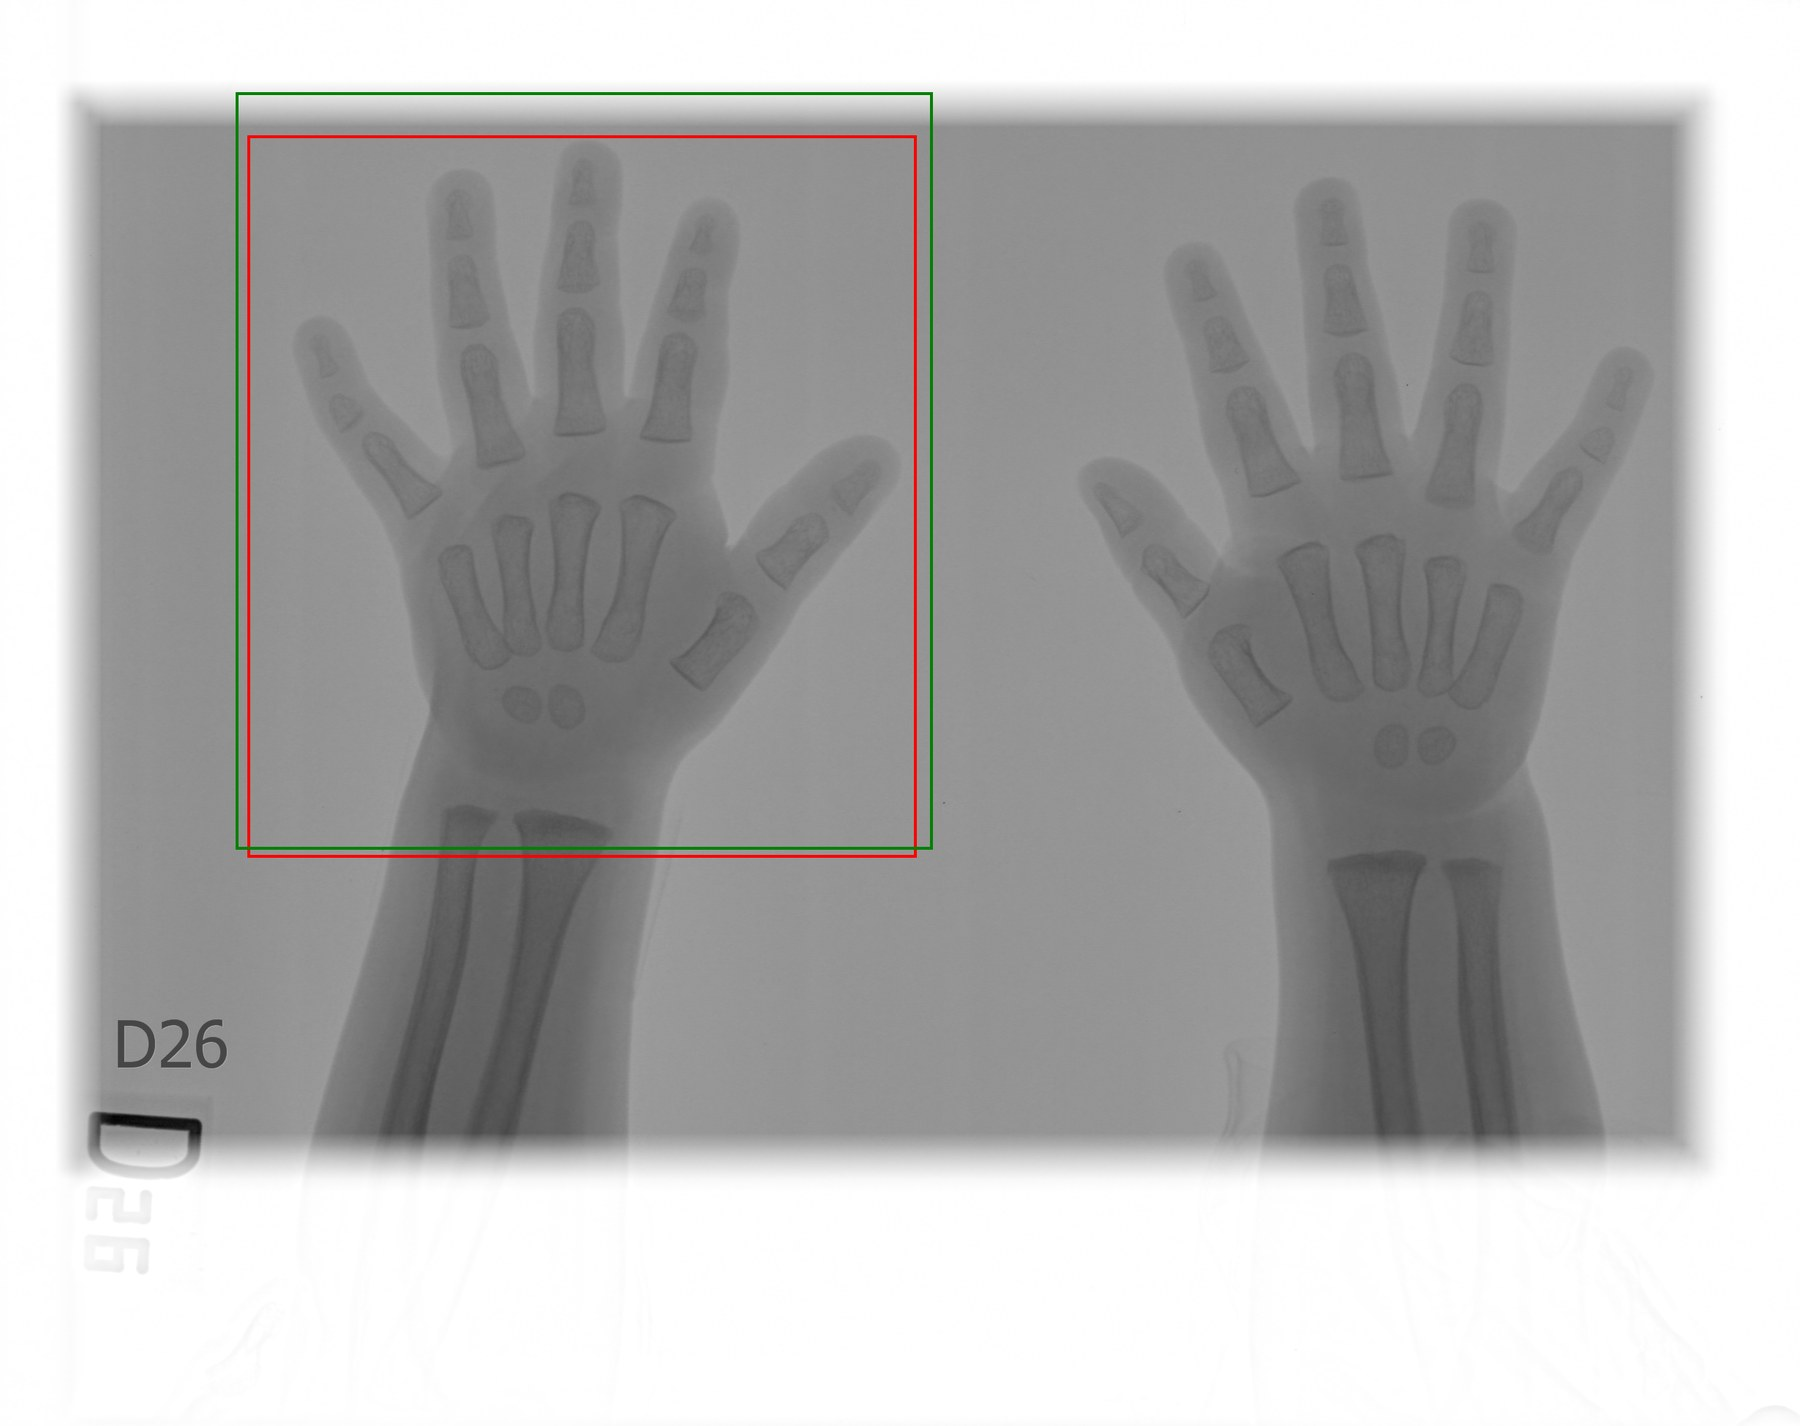
\includegraphics[width=0.32\textwidth]{figure/esempiobbox2.jpg}\hfill
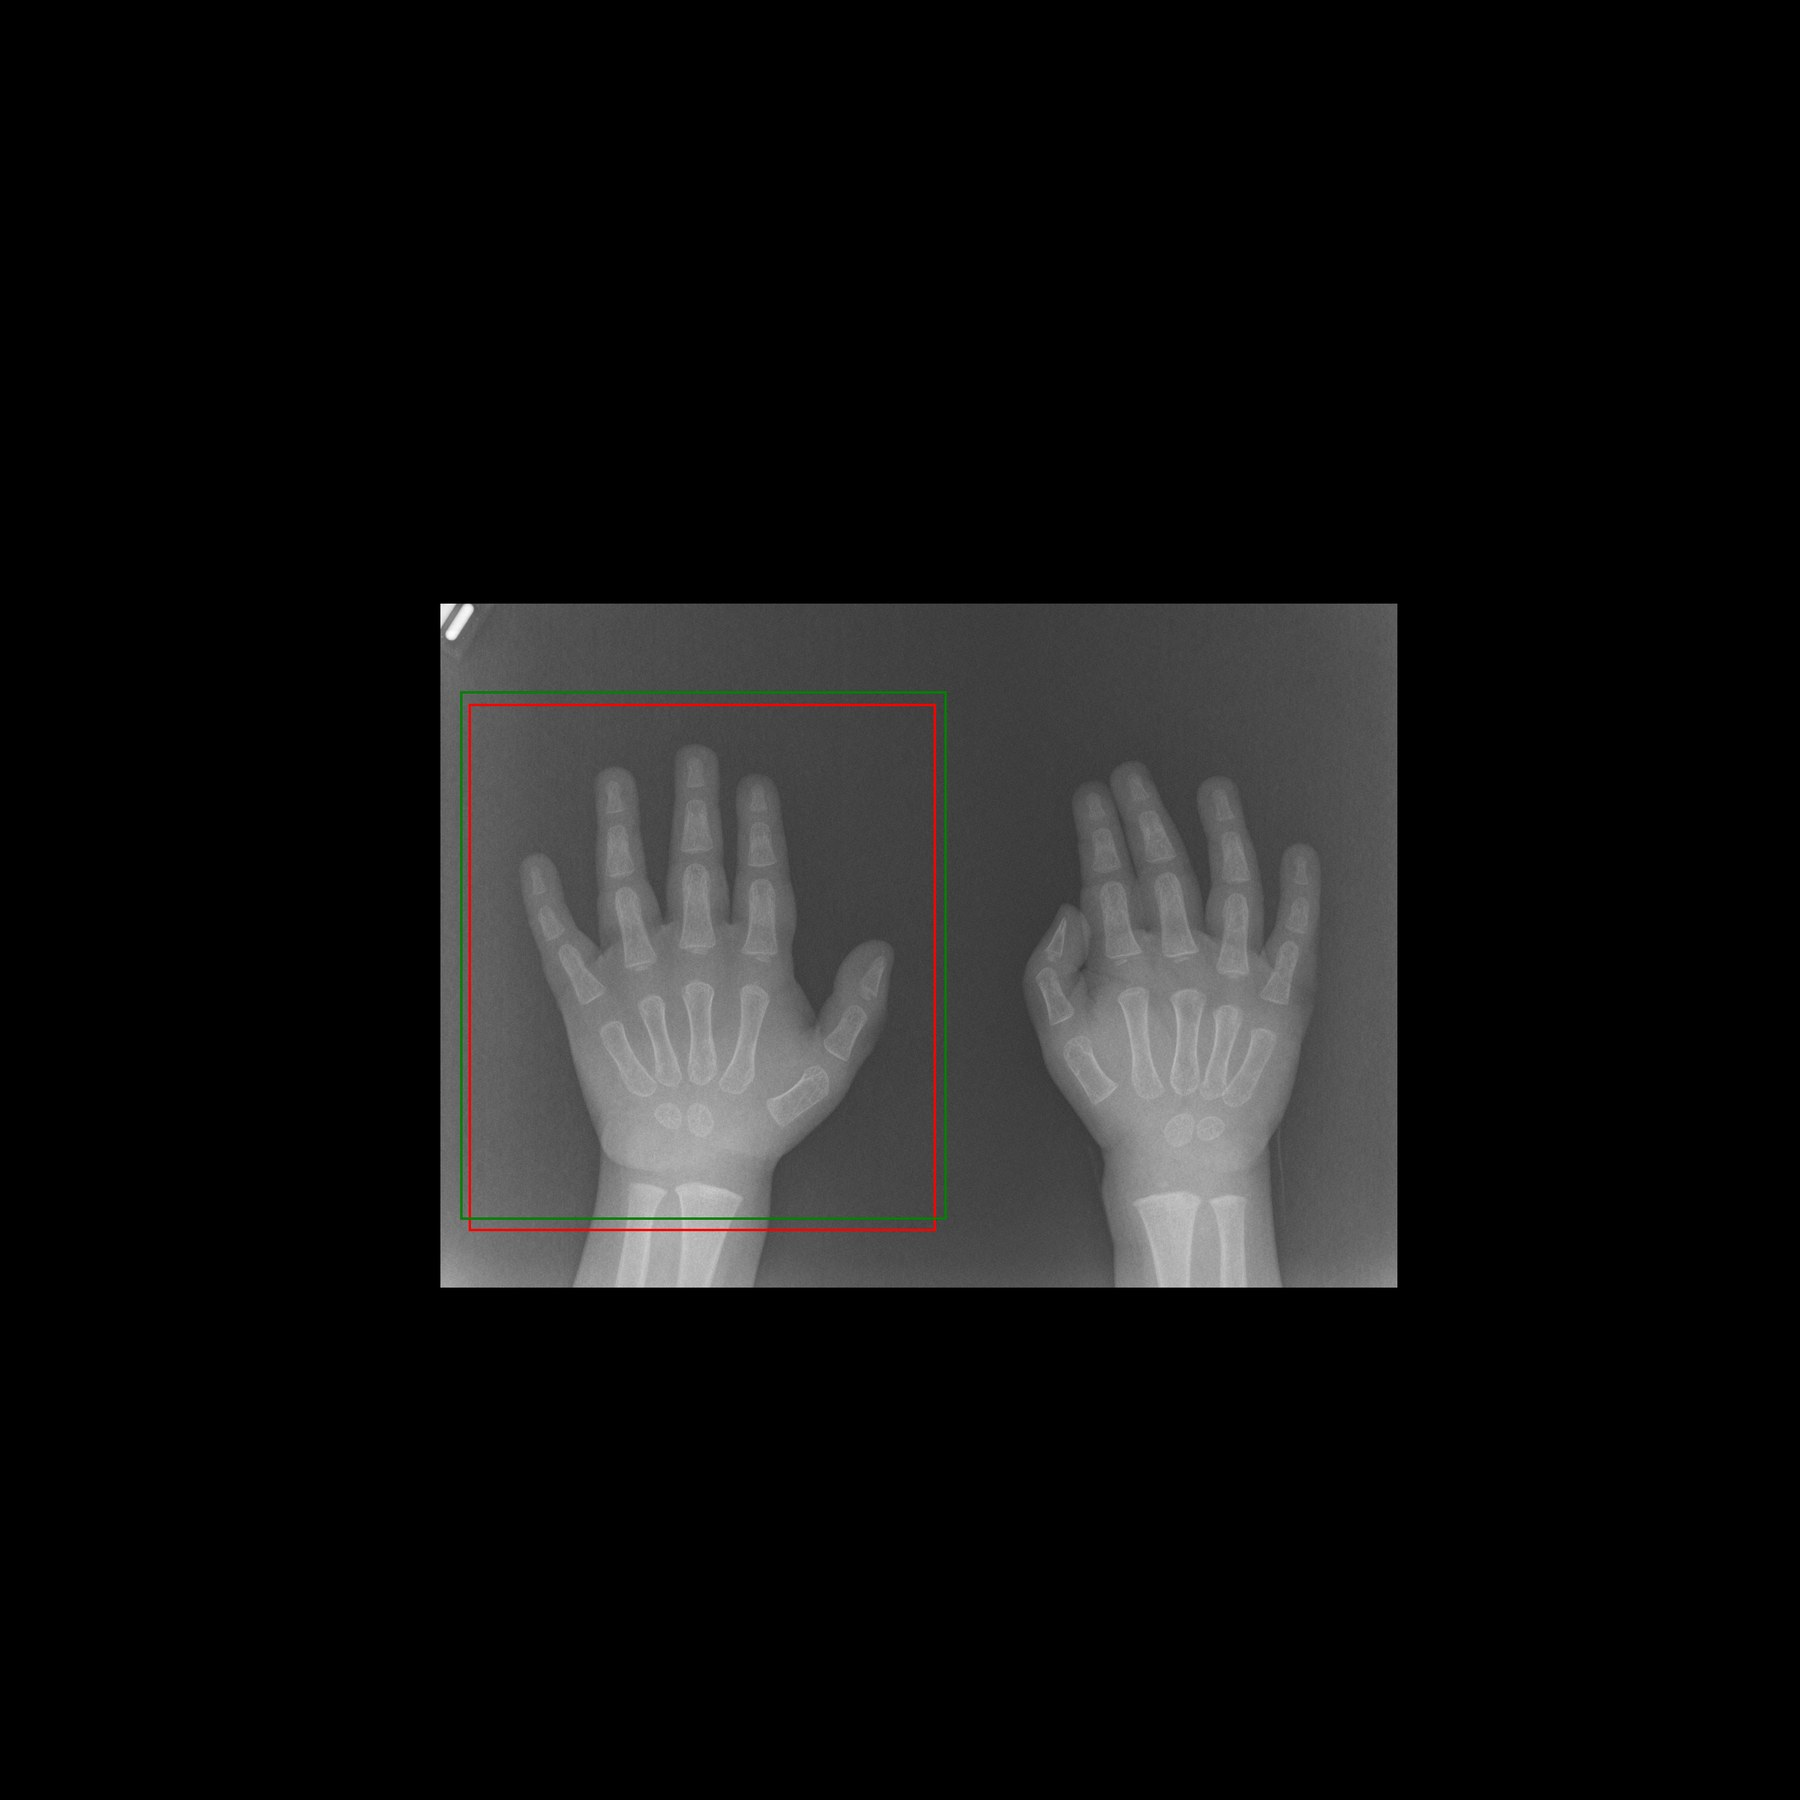
\includegraphics[width=0.32\textwidth]{figure/esempiobbox3.jpg}
\caption{Esempi di bounding box predetta (rossa) e ground truth (verde) sul test set.}
\label{fig:esempi_bbox}
\end{figure}

\section{Keypoint Estimation}
\label{sec:risultati_keypoint}

Le quattro varianti di modello descritte in
Sez.~\ref{sec:varianti_modello} sono state valutate su tutti e tre gli
split, in tre modalità di input: \texttt{full} (immagine intera),
\texttt{gt\_crop} (crop con bounding box ground truth) e
\texttt{det\_crop} (crop con bounding box predetta dal modello di
detection, Sez.~\ref{sec:hand_detection}). I risultati riportati usano i
sigma OKS reali del paper (Tabella~\ref{tab:sigma_oks}).

\begin{table}[htbp]
\centering
\caption{Risultati di keypoint estimation, sigma OKS reali. La mAP è calcolata su soglie di OKS, non di IoU (Sez.~\ref{sec:iou_map}). Le celle in cui la modalità di valutazione coincide con il dominio di training del modello sono evidenziate concettualmente nel testo.}
\label{tab:risultati_keypoint_completo}
\smallskip
\small
\begin{tabular}{llccccc}
\toprule
Split & Model & Mode & mAP@[.5:.95] & mAP@.50 & mAP@.75 & mAR@[.5:.95] \\
\midrule
Test & full & full & 0.6986 & 0.9702 & 0.9061 & 0.7456 \\
Test & full & gt\_crop & 0.5153 & 0.8113 & 0.5550 & 0.5608 \\
Test & full & det\_crop & 0.5407 & 0.8964 & 0.5887 & 0.5937 \\
Test & gt\_crop & full & 0.0856 & 0.2446 & 0.0484 & 0.1013 \\
Test & gt\_crop & gt\_crop & 0.7037 & 0.9619 & 0.9239 & 0.7456 \\
Test & gt\_crop & det\_crop & 0.7205 & 0.9713 & 0.9472 & 0.7620 \\
Test & mirrored & full & 0.0619 & 0.1461 & 0.0235 & 0.0886 \\
Test & mirrored & gt\_crop & 0.6404 & 0.9527 & 0.8030 & 0.6924 \\
Test & mirrored & det\_crop & 0.6433 & 0.9662 & 0.8240 & 0.6924 \\
Test & mirrored\_full & full & 0.7004 & 0.9702 & 0.9183 & 0.7582 \\
Test & mirrored\_full & gt\_crop & 0.5267 & 0.9291 & 0.5707 & 0.5772 \\
Test & mirrored\_full & det\_crop & 0.5606 & 0.9322 & 0.6470 & 0.6089 \\
\bottomrule
\end{tabular}
\end{table}

Dai risultati emergono tre osservazioni principali.

Innanzitutto, la mAP dipende fortemente dalla coerenza tra dominio di
valutazione e dominio di training: ogni modello ottiene le prestazioni
migliori quando valutato nella modalità corrispondente al proprio
addestramento. Il caso più estremo è \texttt{gt\_crop} valutato in
modalità \texttt{full} (mAP@[.5:.95] = 0.086 sul test set, contro 0.704
nel proprio dominio): il modello non ha mai visto, in training, un
target di bounding box diverso dall'intero crop, e di conseguenza non
ha mai imparato a localizzare la mano in un contesto più ampio.

In secondo luogo, tra le quattro varianti \texttt{mirrored\_full} è
quella che si comporta in modo più equilibrato tra i domini: mantiene
prestazioni ragionevoli anche fuori dal proprio dominio primario
(mAP@[.5:.95] $\approx$ 0.53--0.56 su crop, sul test set), contro il
quasi totale collasso di \texttt{gt\_crop} e \texttt{mirrored} in
modalità \texttt{full}. Questo è compatibile con l'ipotesi alla base
della sua progettazione (Sez.~\ref{sec:varianti_modello}); i dati
disponibili non permettono però di isolare quanto di questo vantaggio
derivi dallo specchiamento in sé e quanto dal semplice raddoppio dei
dati di training che esso comporta.

Infine, questo comportamento più equilibrato comporta ormai un costo
marginale: nel proprio dominio nativo \texttt{mirrored\_full} raggiunge
un mAP@[.5:.95] di 0.700, quasi allo stesso livello del picco di
\texttt{gt\_crop} (0.704) e nettamente superiore a quello di
\texttt{mirrored} (0.640) in modalità \texttt{gt\_crop}. Le varianti
allenate su crop restano leggermente più precise quando è disponibile
una bounding box di alta qualità a monte, ma il divario si è ridotto a
pochi millesimi; \texttt{mirrored\_full} resta inoltre l'unica in grado
di funzionare direttamente sull'immagine intera, gestendo entrambe le
mani in un unico passaggio, senza necessitare di una fase di
localizzazione separata.

Confrontando con il paper BoNet~\cite{escobar2019bonet} (mAP@[.5:.95]
$=$ 0.814 con bounding box ground truth sul dataset RHPE, sull'intero
training set), i risultati ottenuti su un sottoinsieme di 250 immagini
(\texttt{gt\_crop} in modalità \texttt{gt\_crop}: 0.704; \texttt{mirrored}
in modalità \texttt{gt\_crop}: 0.640) risultano inferiori a quelli
riportati da BoNet. La differenza va però interpretata tenendo conto
sia della significativa riduzione del dataset di training, sia
dell'architettura diversa adottata per la keypoint estimation
(Keypoint R-CNN anziché Simple Baselines,
Sez.~\ref{sec:keypoint_estimation}): non si tratta quindi di un
confronto perfettamente controllato.

\begin{figure}[htbp]
\centering
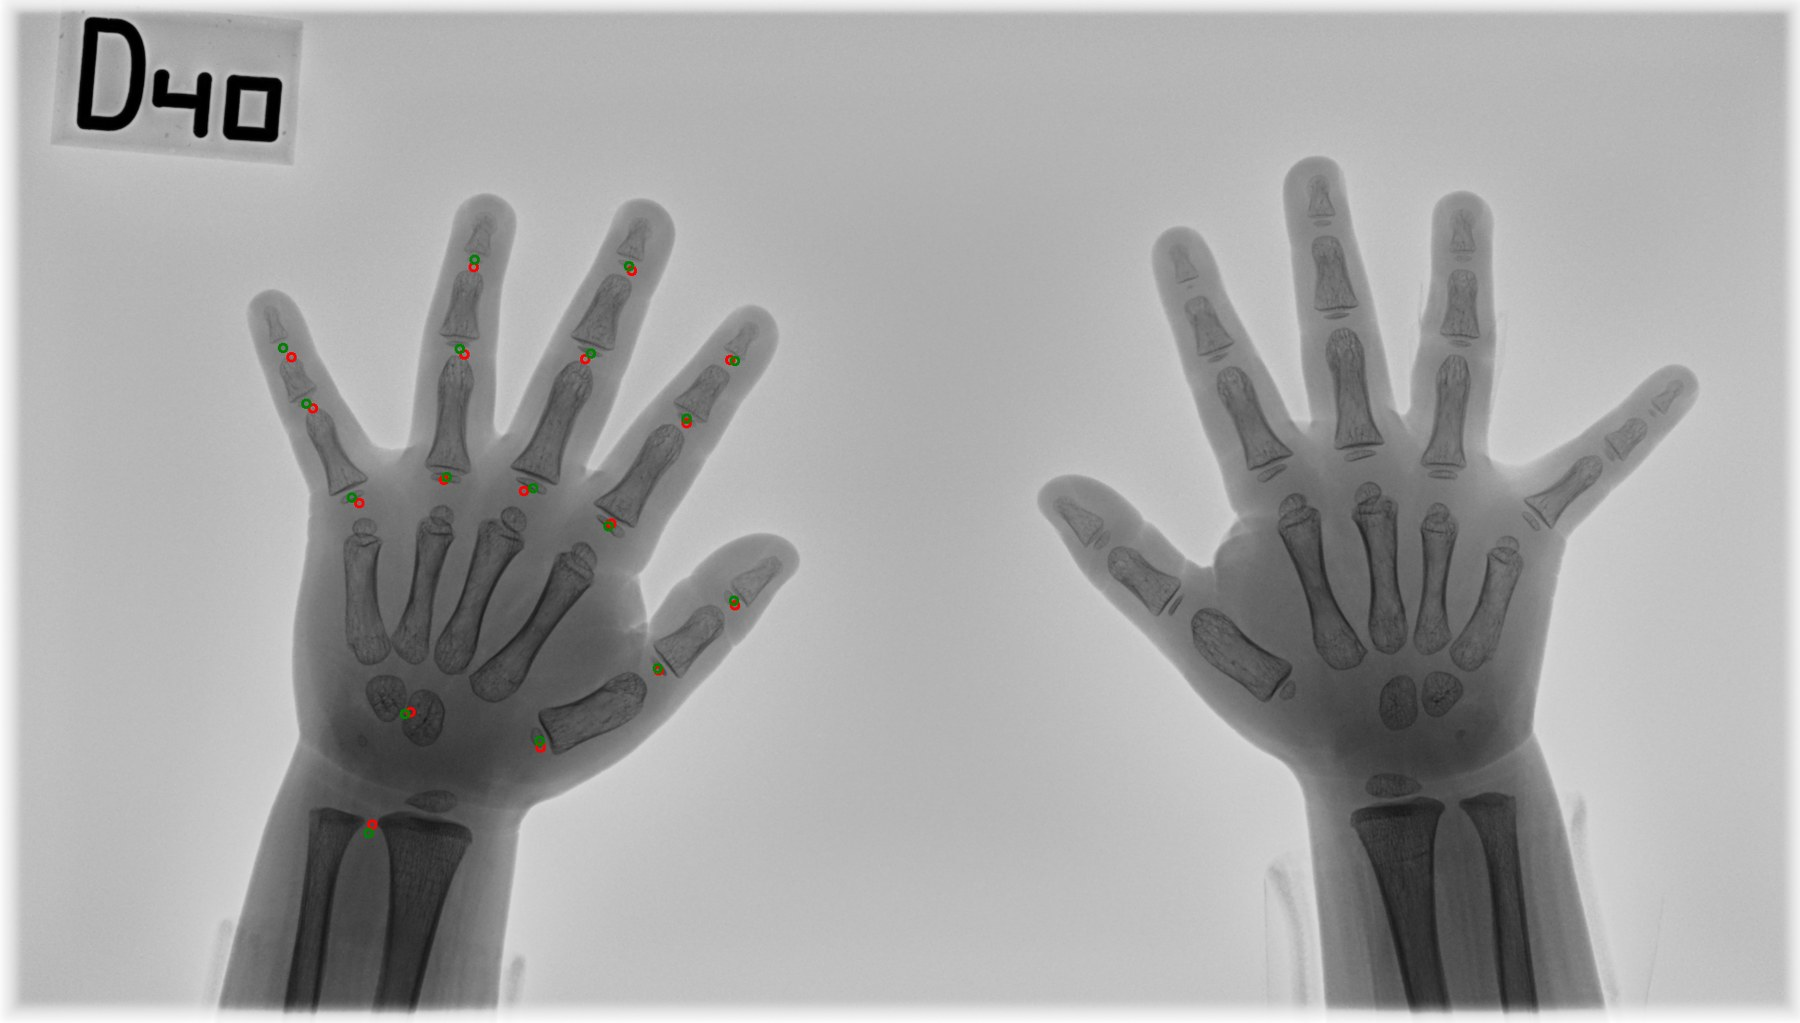
\includegraphics[width=0.48\textwidth]{figure/kpfullmodefull.jpg}\hfill
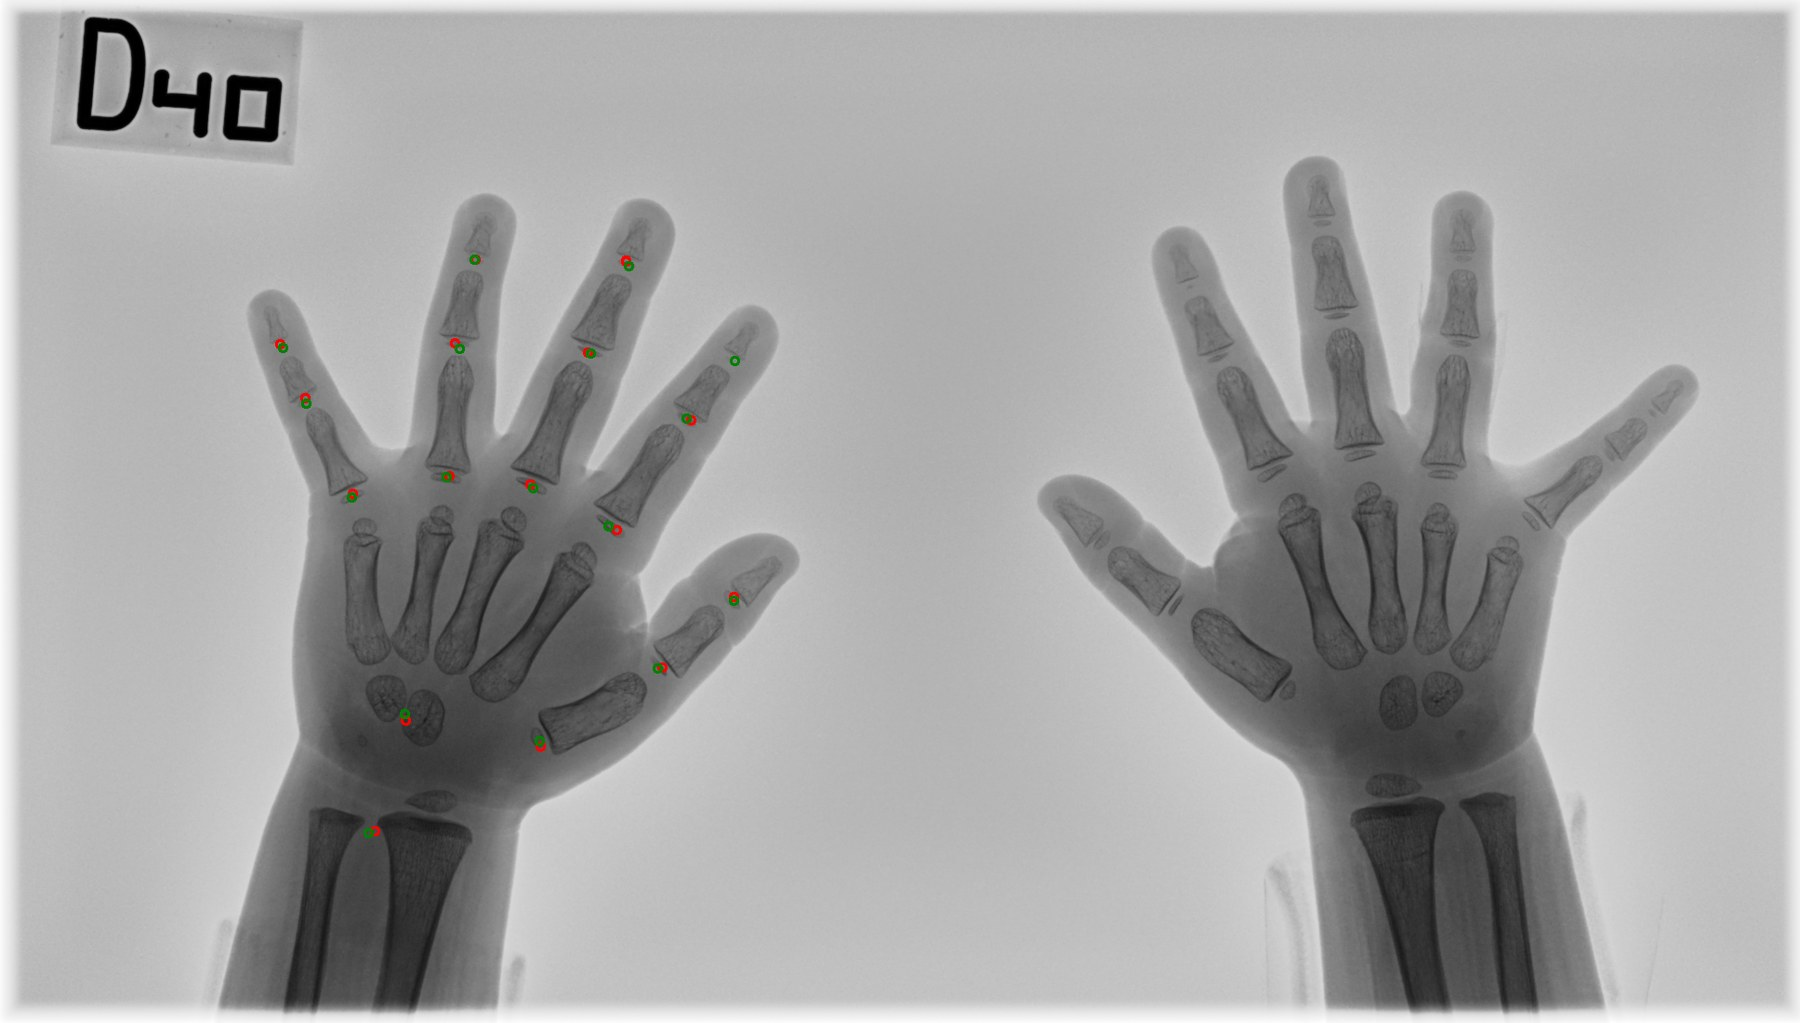
\includegraphics[width=0.48\textwidth]{figure/kpgtcropmodegtcrop.jpg}\\[1em]
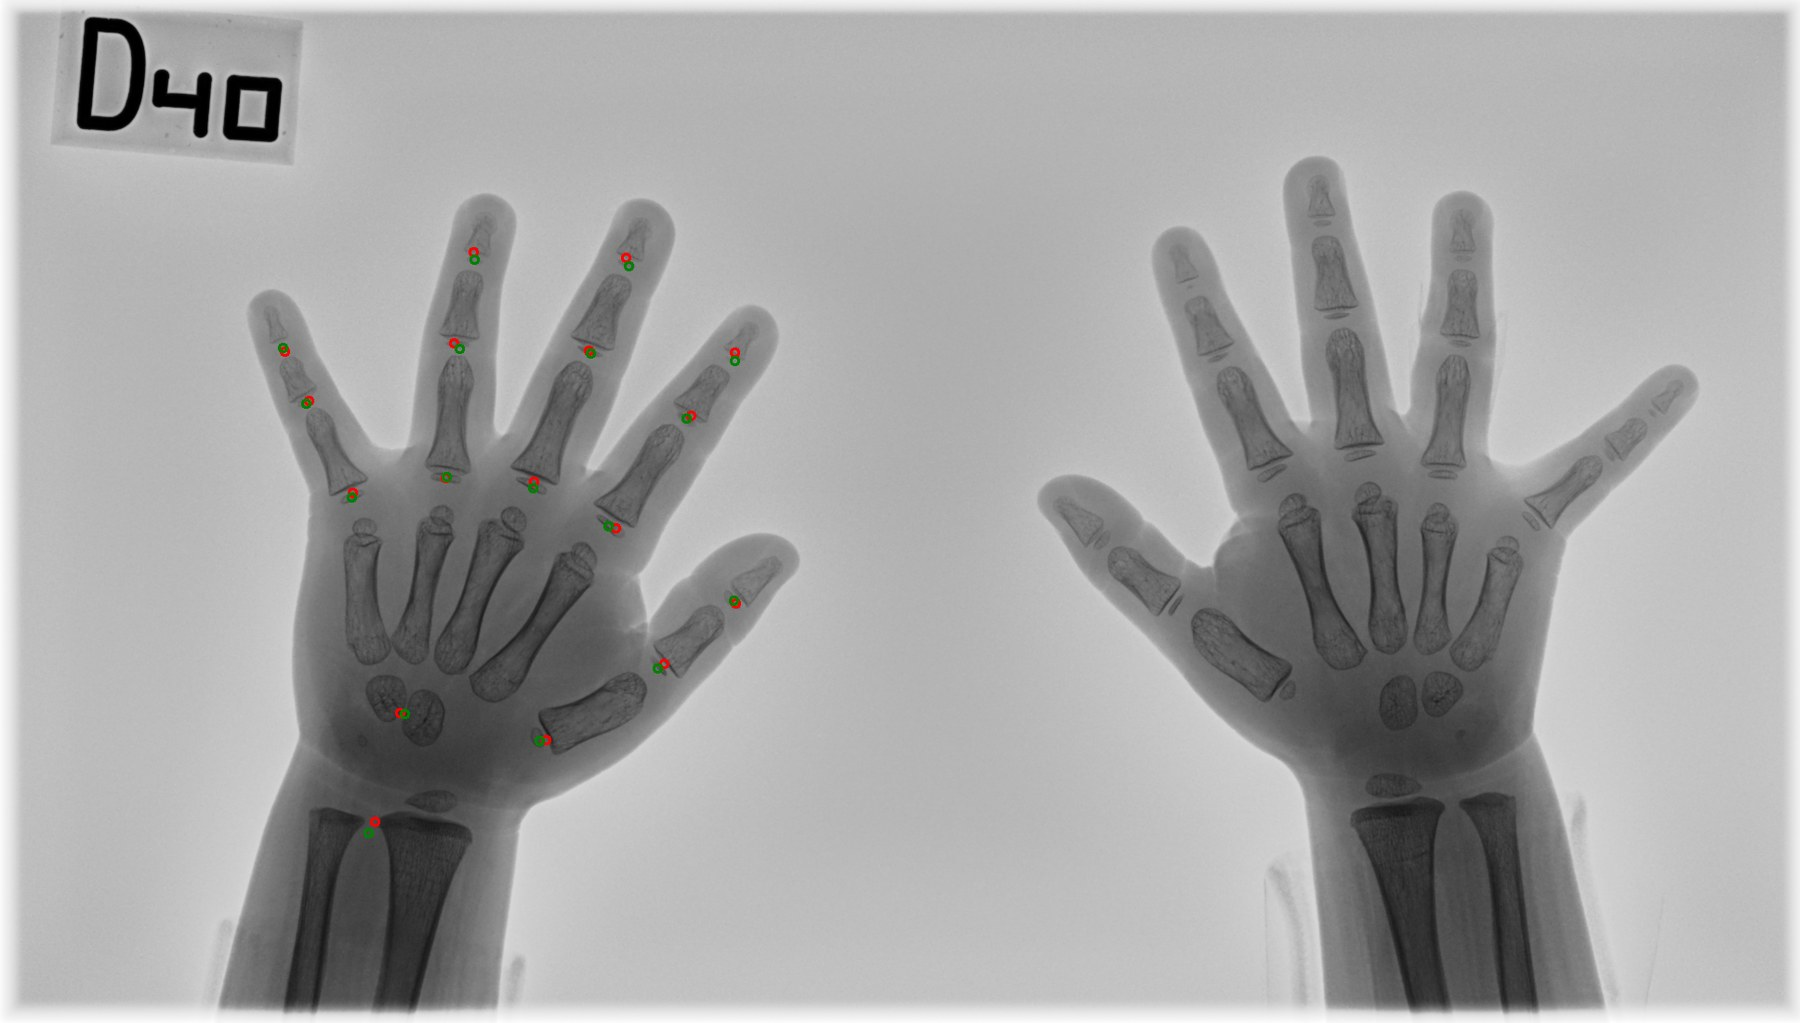
\includegraphics[width=0.48\textwidth]{figure/kpgtcropmodedetcrop.jpg}\hfill
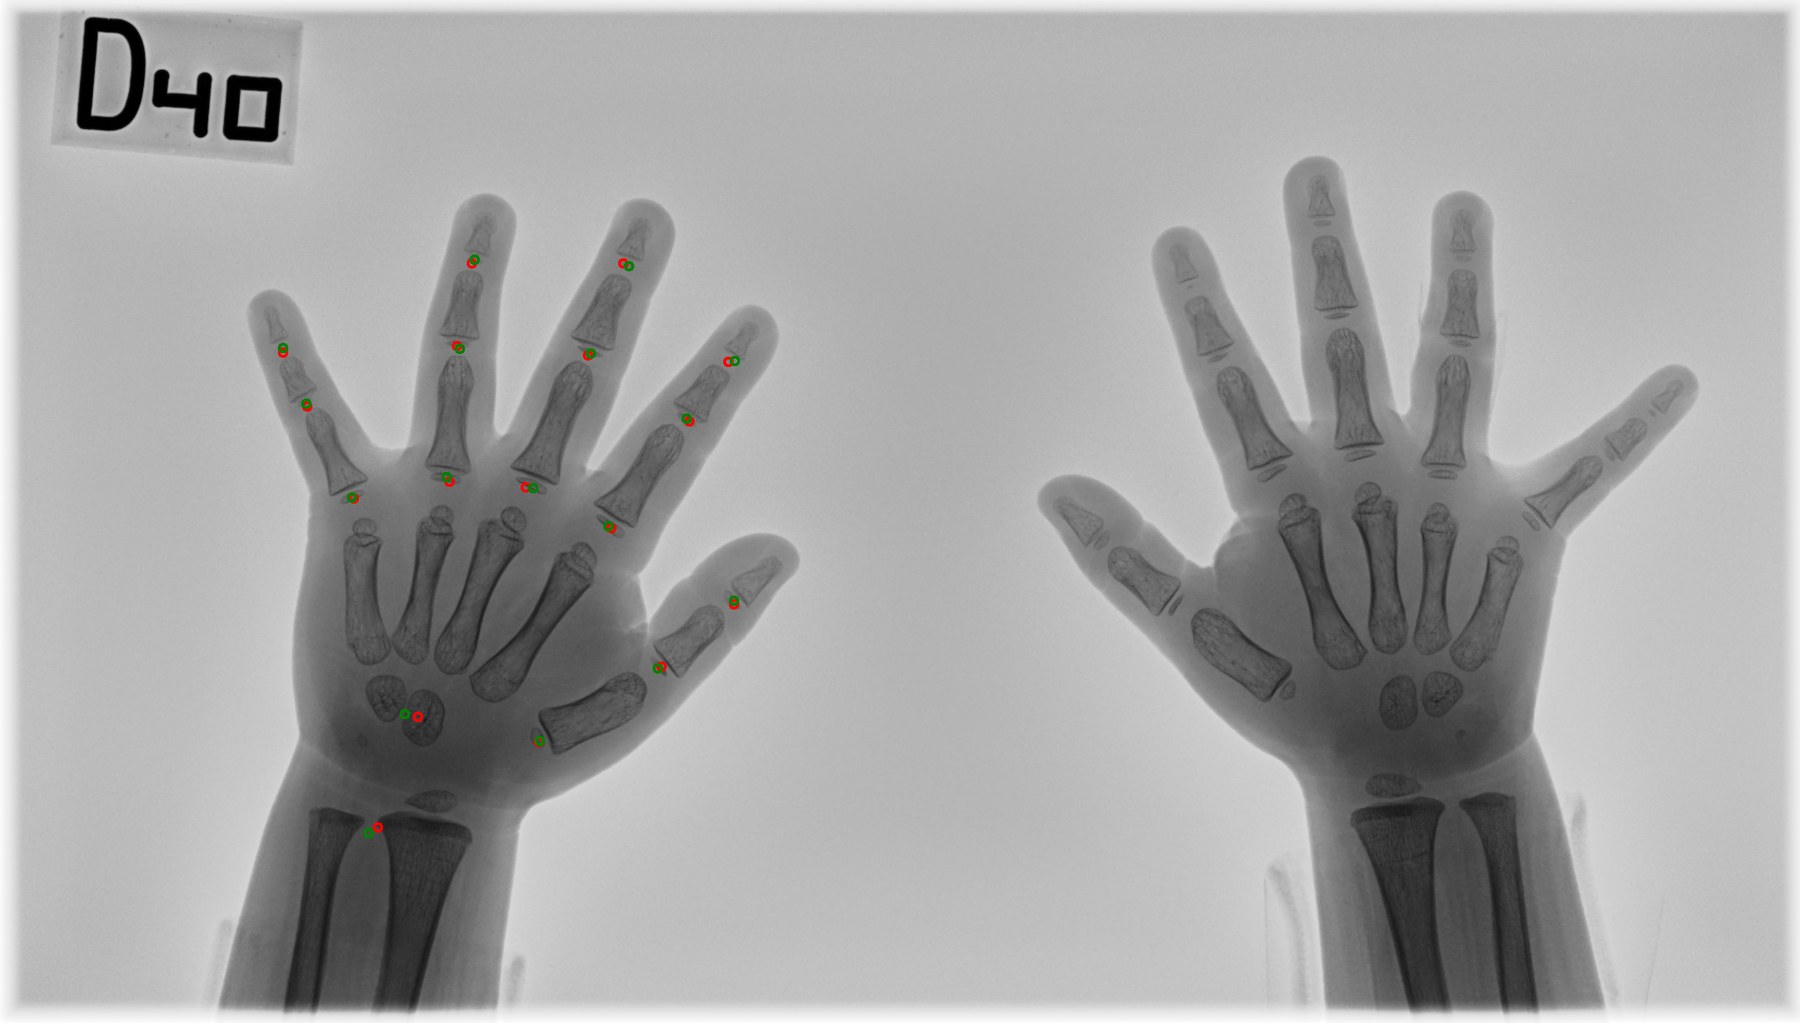
\includegraphics[width=0.48\textwidth]{figure/kpmirroredfullmodefull1.jpg}
\caption{Esempi di keypoint predetti (rossi) e ground truth (verdi) per quattro
combinazioni modello/modalità: \texttt{full}/\texttt{full} (in alto a
sinistra), \texttt{gt\_crop}/\texttt{gt\_crop} (in alto a destra),
\texttt{gt\_crop}/\texttt{det\_crop} (in basso a sinistra),
\texttt{mirrored\_full}/\texttt{full} (in basso a destra).}
\label{fig:esempi_keypoint}
\end{figure}

\subsection{Retraining di \texttt{gt\_crop} sul dataset completo}
\label{sec:retraining_gt_crop_full}

Poiché \texttt{gt\_crop} è la variante che più fedelmente replica la
metodologia di BoNet (Sez.~\ref{sec:varianti_modello}), è stata
riallenata sull'intero training set RHPE (5.492 immagini, contro le 250
del sottoinsieme stratificato), utilizzando il criterio di validazione
basato sulla loss descritto in Sez.~\ref{sec:keypoint_estimation}. Una
seconda versione è stata inoltre allenata con la data augmentation
descritta nella stessa sezione (rotazione e scala casuali). I risultati
sul test set sono riportati in
Tabella~\ref{tab:risultati_gt_crop_fulldata}.

\begin{table}[H]
\centering
\caption{Risultati di \texttt{gt\_crop} riallenato sul dataset completo,
con e senza data augmentation. Confronto diretto con le righe
\texttt{gt\_crop} di Tabella~\ref{tab:risultati_keypoint_completo}
(sottoinsieme da 250 immagini).}
\label{tab:risultati_gt_crop_fulldata}
\smallskip
\small
\begin{tabular}{lccccc}
\toprule
Mode & Augmentation & mAP@[.5:.95] & mAP@.50 & mAP@.75 & mAR@[.5:.95] \\
\midrule
full      & no & 0.1043 & 0.2365 & 0.0847 & 0.1595 \\
full      & sì & 0.4017 & 0.7233 & 0.4017 & 0.4570 \\
gt\_crop  & no & 0.7508 & 0.9587 & 0.9484 & 0.7937 \\
gt\_crop  & sì & 0.7699 & 0.9690 & 0.9563 & 0.8013 \\
det\_crop & no & 0.7330 & 0.9685 & 0.9553 & 0.7899 \\
det\_crop & sì & 0.7913 & 0.9741 & 0.9616 & 0.8278 \\
\bottomrule
\end{tabular}
\end{table}

Rispetto al sottoinsieme da 250 immagini
(Tabella~\ref{tab:risultati_keypoint_completo}), l'addestramento sul
dataset completo migliora le prestazioni ma non in modo decisivo:
mAP@[.5:.95] passa da 0.7037 a 0.7508 in modalità \texttt{gt\_crop}
(+0.047) e da 0.7205 a 0.7330 in modalità \texttt{det\_crop} (+0.013).
Il pattern è interessante: mAP@.50 non migliora, mentre mAP@.75 e
mAR@[.5:.95] migliorano in entrambe le modalità. Il modello, già con 250
immagini, aveva imparato a localizzare i keypoint approssimativamente
nella posizione corretta quasi sempre; il margine di miglioramento con
più dati si colloca sulla precisione fine, non sulla capacità di evitare
errori grossolani.

L'aggiunta della data augmentation produce un miglioramento ulteriore,
non uniforme tra le modalità: marginale nel dominio nativo del modello
(\texttt{gt\_crop}: +0.019), più marcato quando l'input si discosta
dalle condizioni di training (\texttt{det\_crop}: +0.058; \texttt{full}:
+0.297 in termini relativi, pur restando un valore assoluto basso).
La spiegazione è geometrica: quando la rotazione casuale
(Sez.~\ref{sec:keypoint_estimation}) ruota il box ground truth, il
nuovo box assiale usato per il crop, il più piccolo rettangolo dritto
che contiene i quattro angoli ruotati, è per costruzione più grande del
box di partenza (tranne che per rotazioni di 0°, 90°, 180°...),
aggiungendo quindi margine ulteriore rispetto a quello già presente
nell'annotazione originale, quale che sia la sua aderenza alla mano; la
componente di scala, al contrario, moltiplica tutte le coordinate per
lo stesso fattore e non altera il margine relativo del crop. Il modello
si allena quindi, per effetto della sola rotazione, su crop
sistematicamente più larghi rispetto all'annotazione di partenza, una
condizione più vicina a quella di un box predetto da un detector, in
genere meno preciso di un'annotazione manuale: il beneficio
dell'augmentation si osserva perciò più chiaramente in modalità
\texttt{det\_crop}, dove questo tipo di margine è già presente
indipendentemente dall'augmentation stessa.

Con la combinazione dataset completo e augmentation, il divario rispetto
al valore riportato da BoNet per RHPE con bounding box ground truth
(mAP@[.5:.95] = 0.814) si riduce da 0.063 a 0.044 (\texttt{gt\_crop} in
modalità \texttt{gt\_crop}: 0.7699). Il confronto approfondito con
questo valore è discusso nel Capitolo~\ref{chap:discussione}.

Le altre tre varianti (\texttt{full}, \texttt{mirrored},
\texttt{mirrored\_full}) non sono state riallenate sul dataset completo;
i valori corrispondenti in Tabella~\ref{tab:risultati_keypoint_completo}
restano quindi quelli ottenuti sul sottoinsieme.

\section{Esplorazione su entrambe le mani: risultati}
\label{sec:esplorazione_dx}

Poiché il test set RHPE non include ground truth per la mano destra, i
quattro approcci descritti in Sez.~\ref{sec:esplorazione_dx_metodo} sono
stati valutati qualitativamente, tramite ispezione visiva delle
predizioni su un campione di 5 immagini di test:

\begin{description}
    \item[v1] Il modello \texttt{full} non generalizza alla ricerca di
    una seconda mano, non avendo mai visto più di una bounding box per
    immagine in training: le detection aggiuntive ottengono punteggi
    molto bassi (0.06--0.13) e in alcuni casi corrispondono a doppioni
    della stessa mano sinistra, non alla destra.
\end{description}

\begin{figure}[H]
\centering
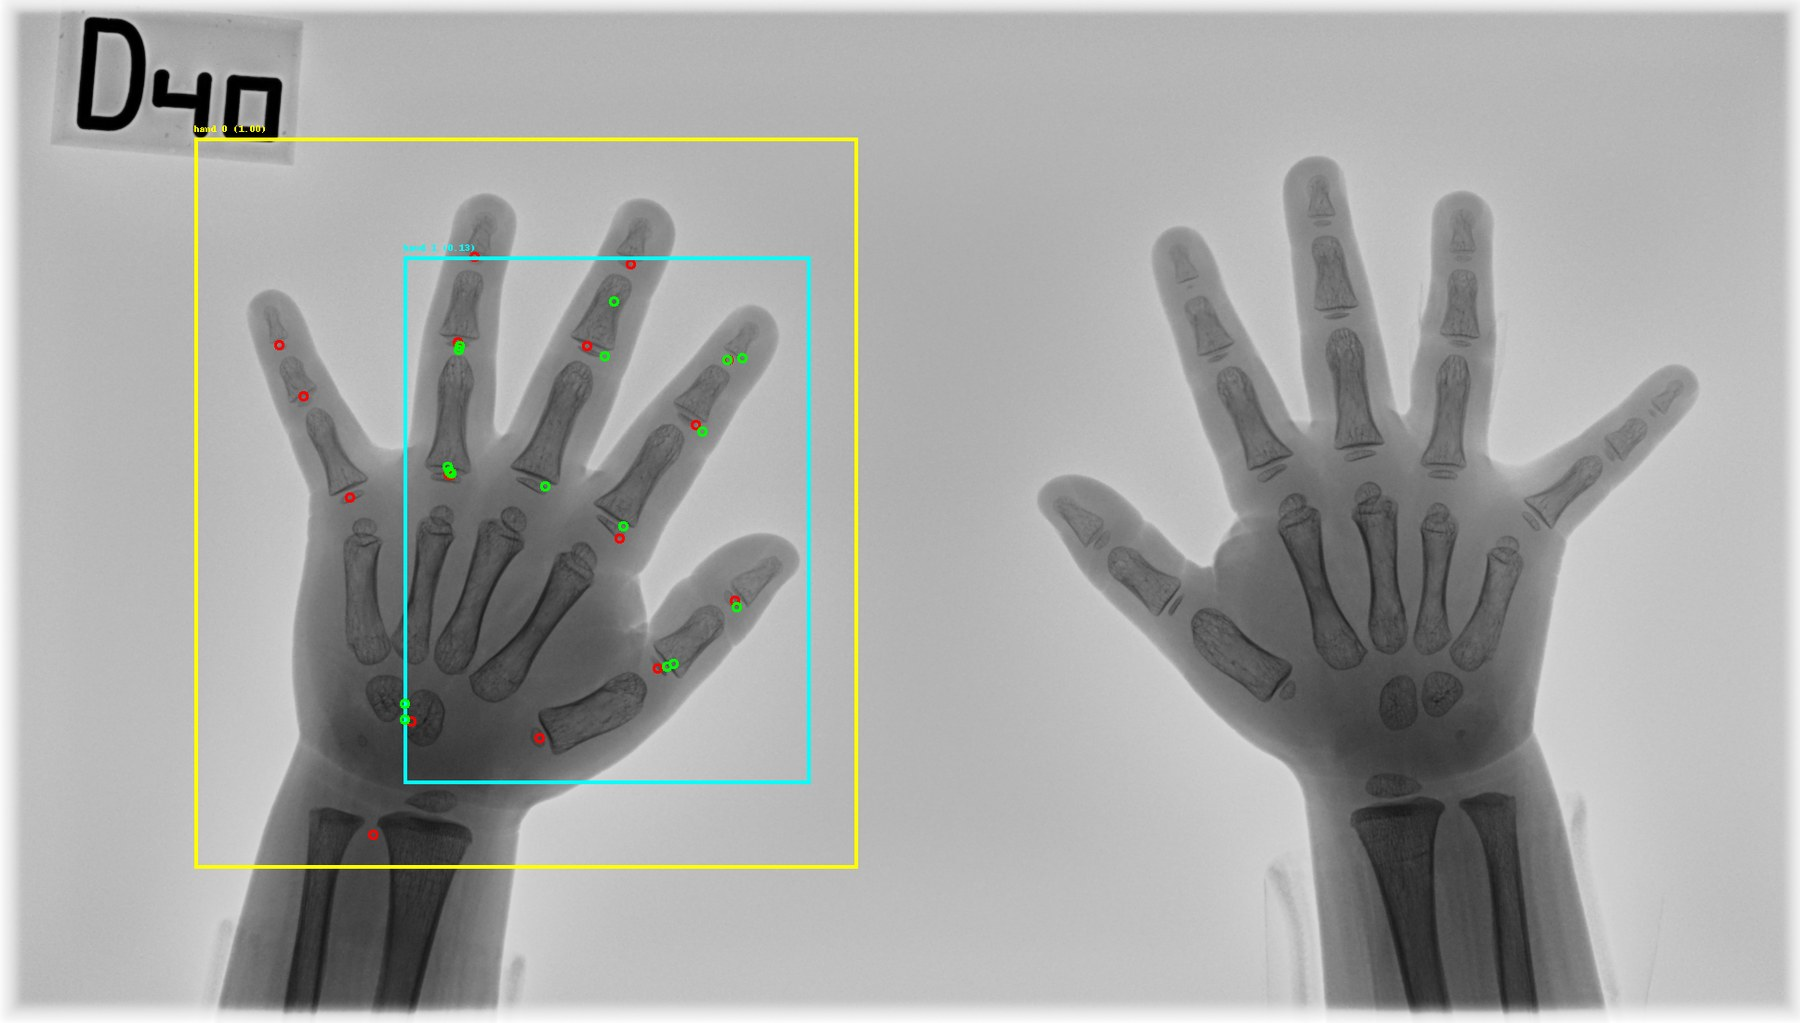
\includegraphics[width=0.48\textwidth]{figure/rhkpv1.jpg}\hfill
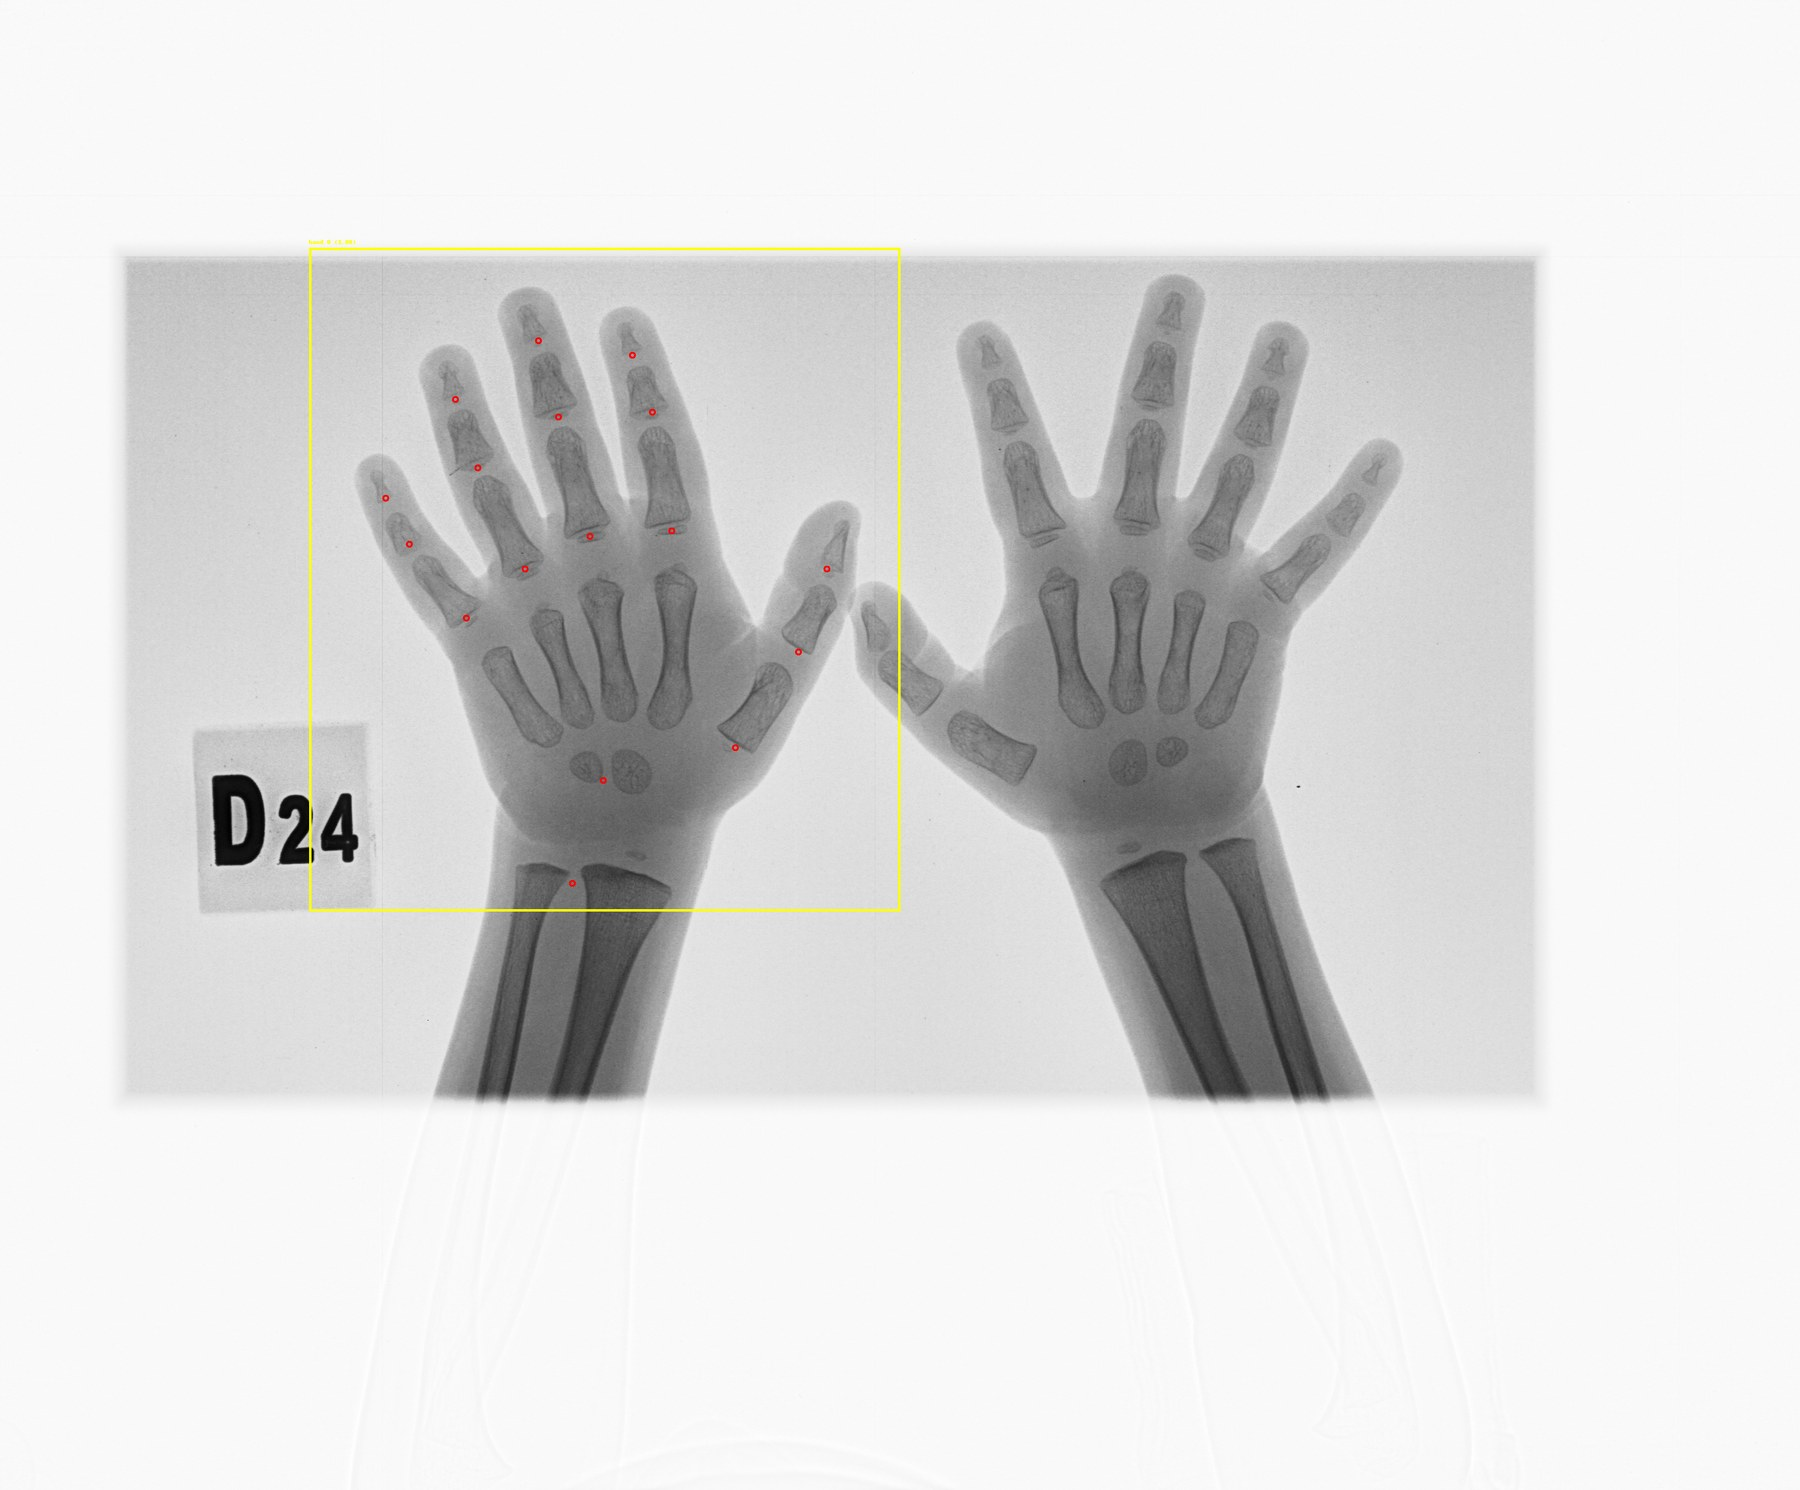
\includegraphics[width=0.48\textwidth]{figure/rhkpv1_2.jpg}
\caption{v1: detection con \texttt{full} sull'immagine intera, keypoint
con \texttt{mirrored}.}
\label{fig:rhkp_v1}
\end{figure}

\begin{description}
    \item[v2] Risultati incostanti: la mano destra viene rilevata con
    buon punteggio in 2 immagini su 5, con punteggio molto basso
    (0.09--0.31, sotto soglia) in altre 2, e nessuna detection nella
    restante.
\end{description}

\begin{figure}[H]
\centering
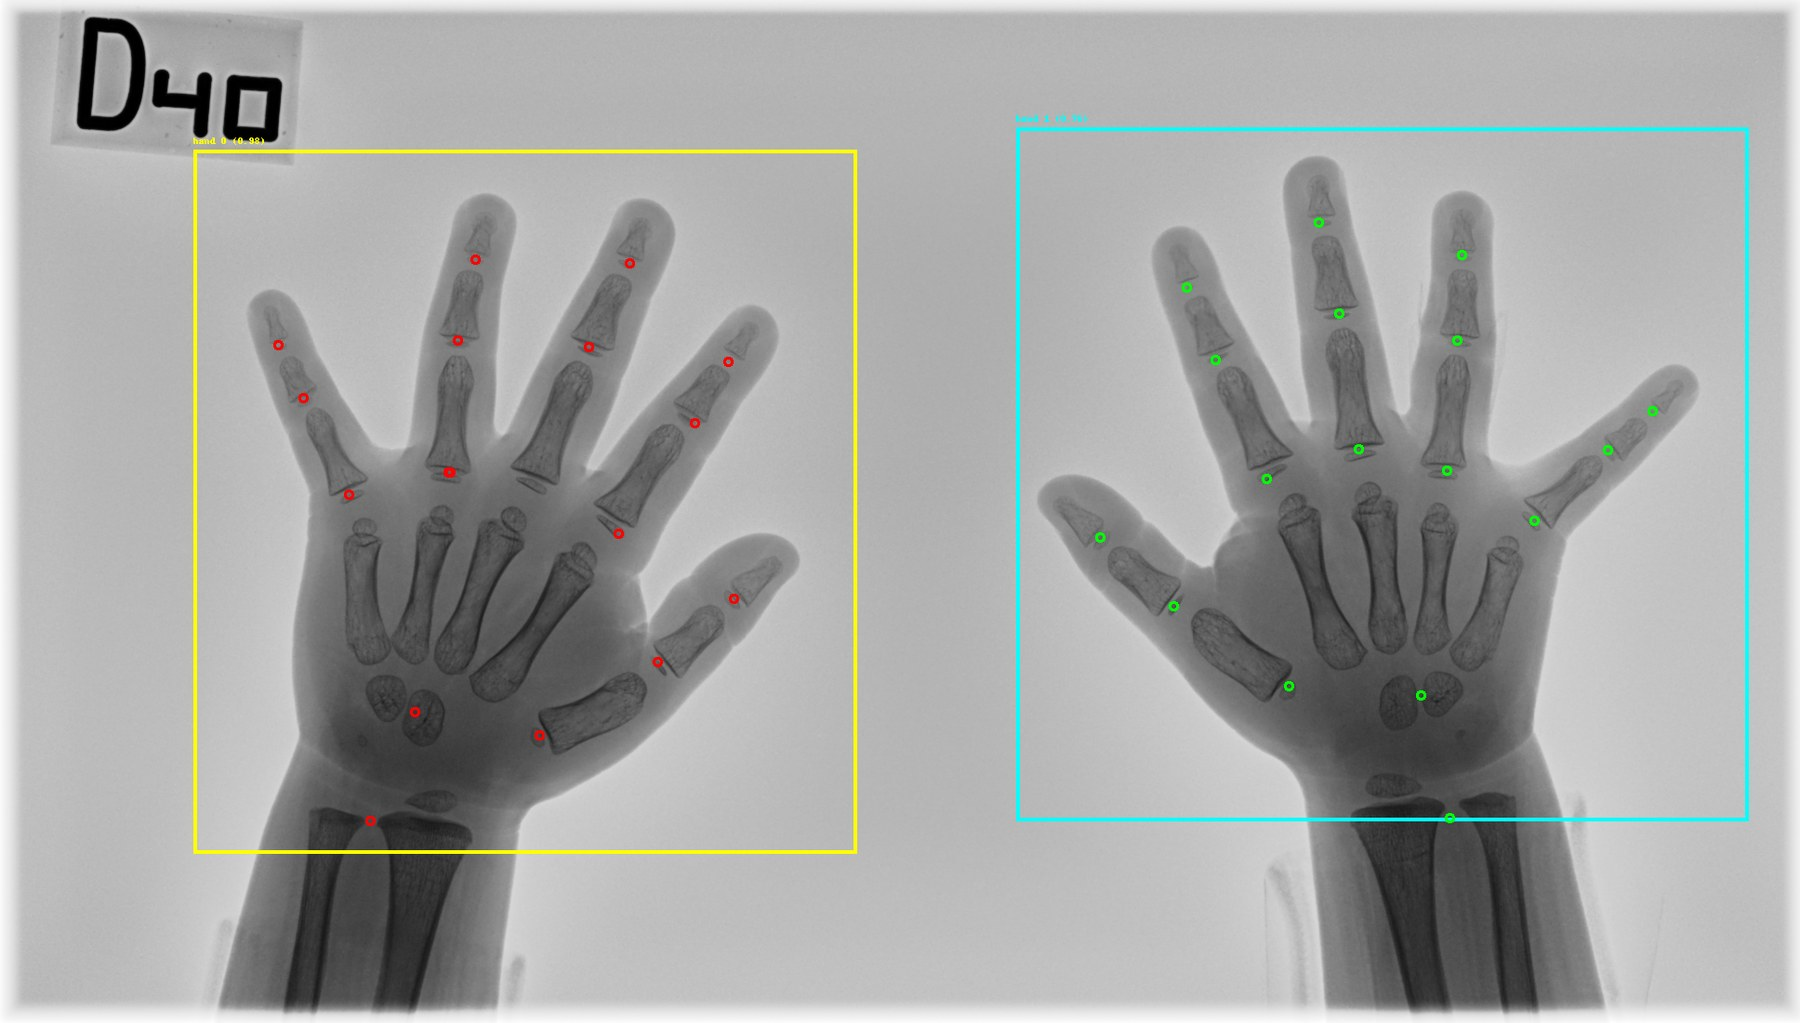
\includegraphics[width=0.48\textwidth]{figure/rhkpv2.jpg}\hfill
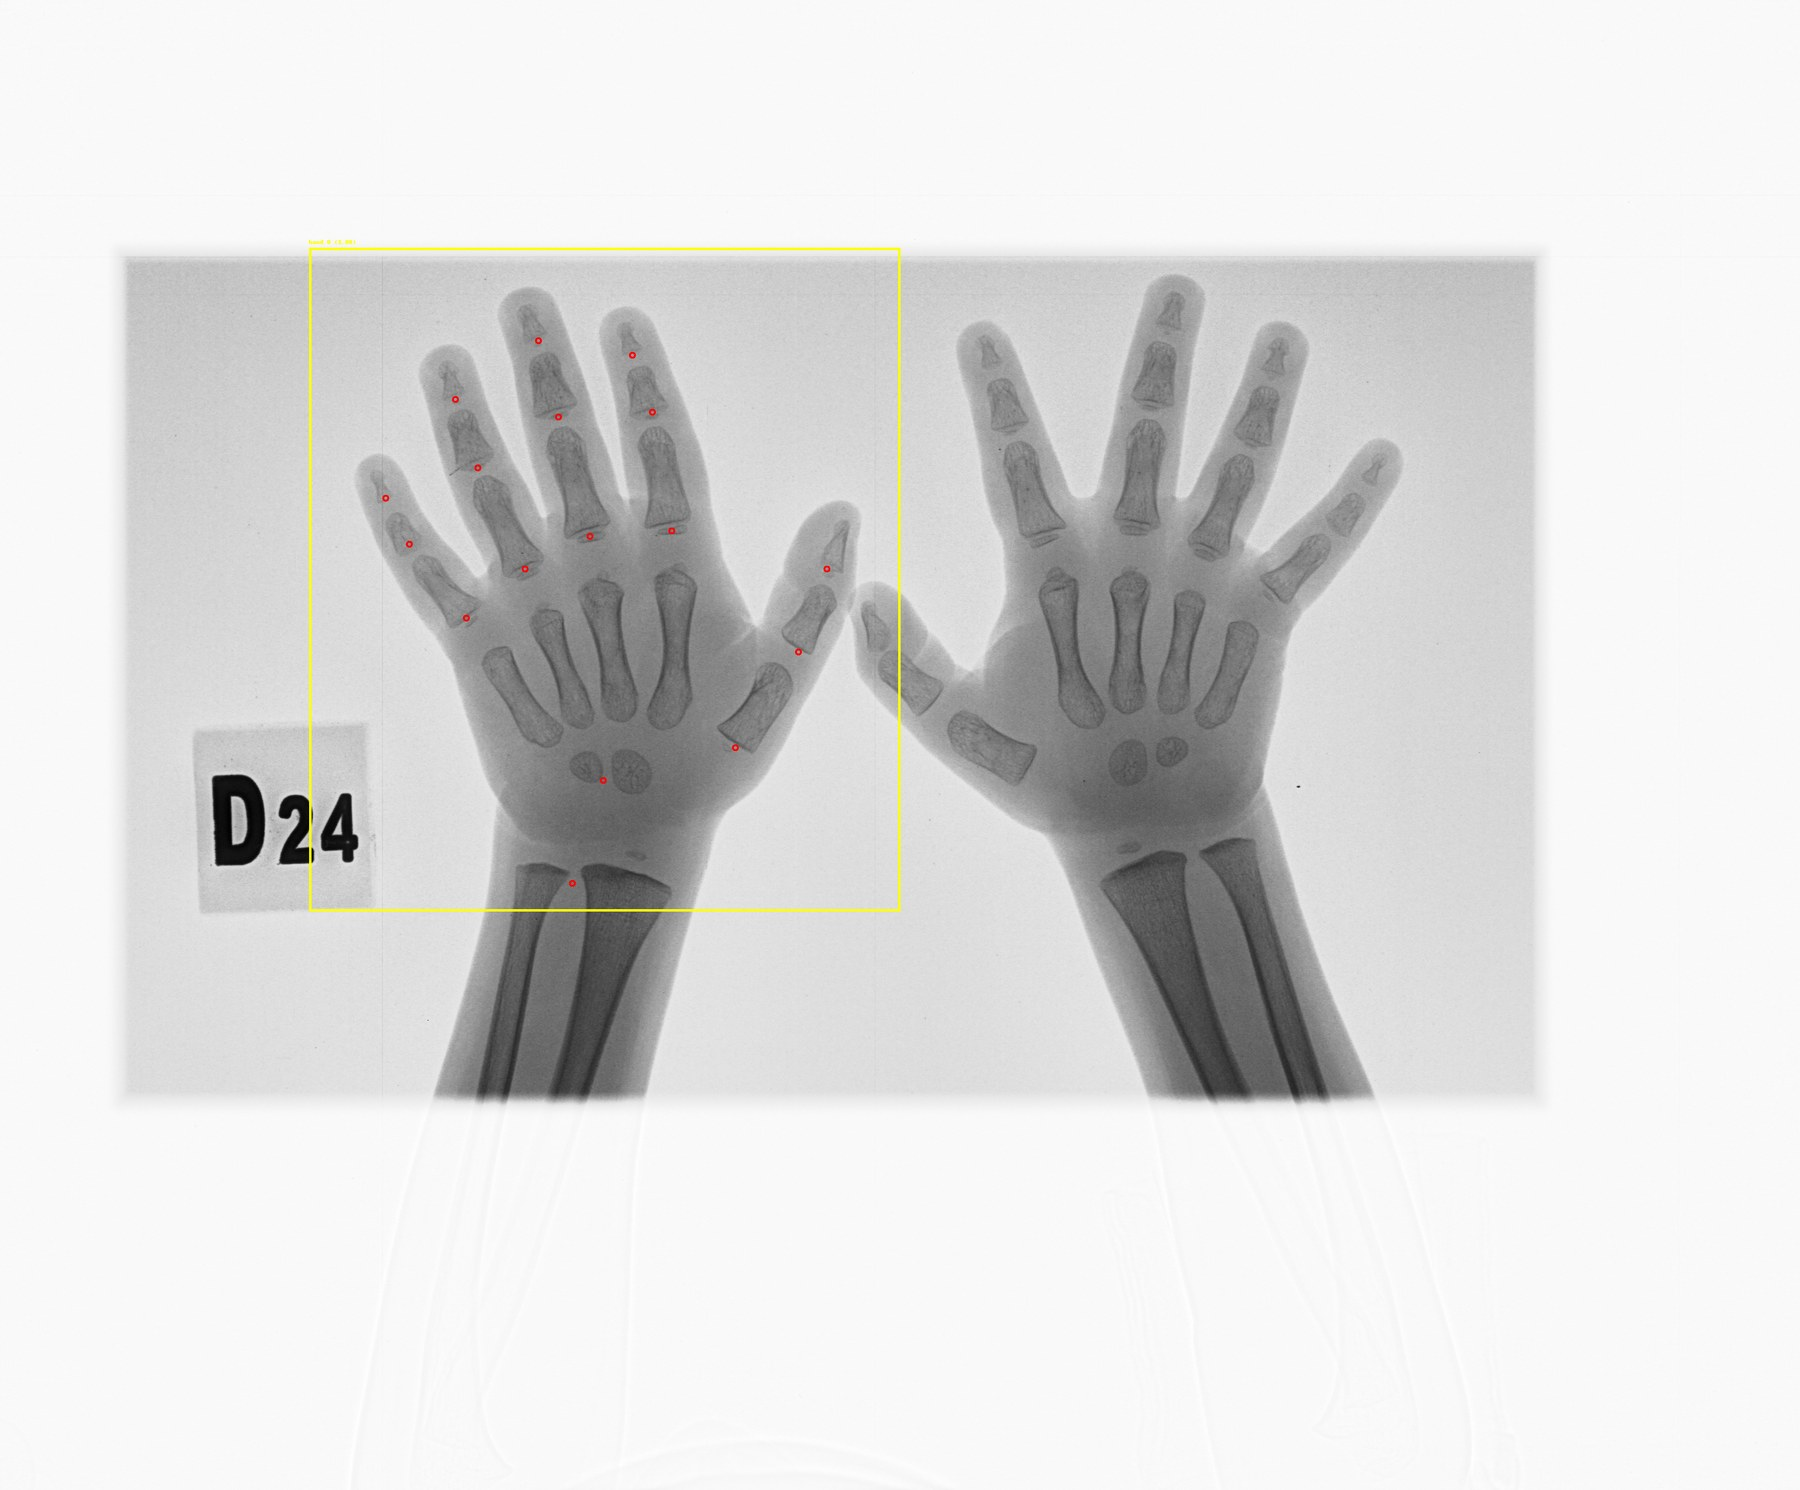
\includegraphics[width=0.48\textwidth]{figure/rhkpv2_2.jpg}
\caption{v2: immagine divisa a metà, detection con \texttt{full} su
ciascuna metà, keypoint con \texttt{mirrored}.}
\label{fig:rhkp_v2}
\end{figure}

\begin{description}
    \item[v3] La detection diventa affidabile su entrambe le metà, con
    punteggi superiori a 0.98 su tutte e 5 le immagini del campione, ma
    a un'ispezione visiva i keypoint predetti appaiono errati su
    entrambe le mani, coerentemente con il limite di generalizzazione
    di \texttt{mirrored} discusso in Sez.~\ref{sec:varianti_modello}.
\end{description}

\begin{figure}[H]
\centering
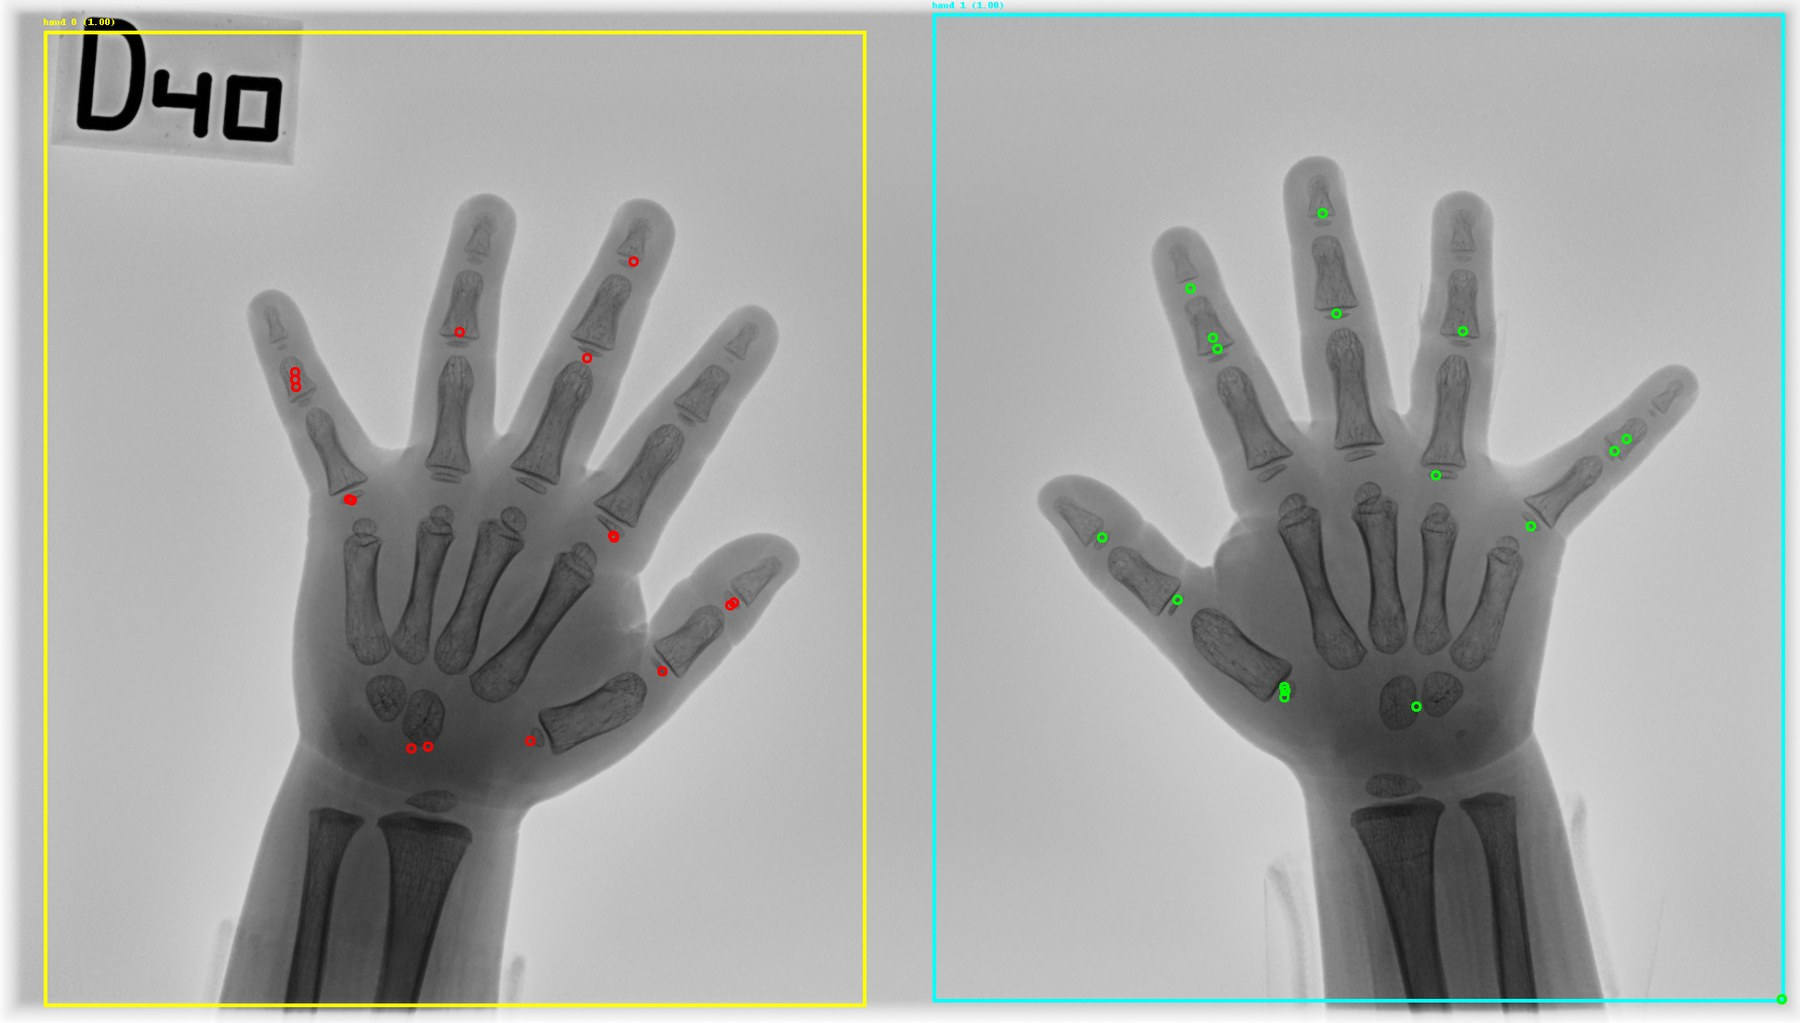
\includegraphics[width=0.48\textwidth]{figure/rhkpv3.jpg}\hfill
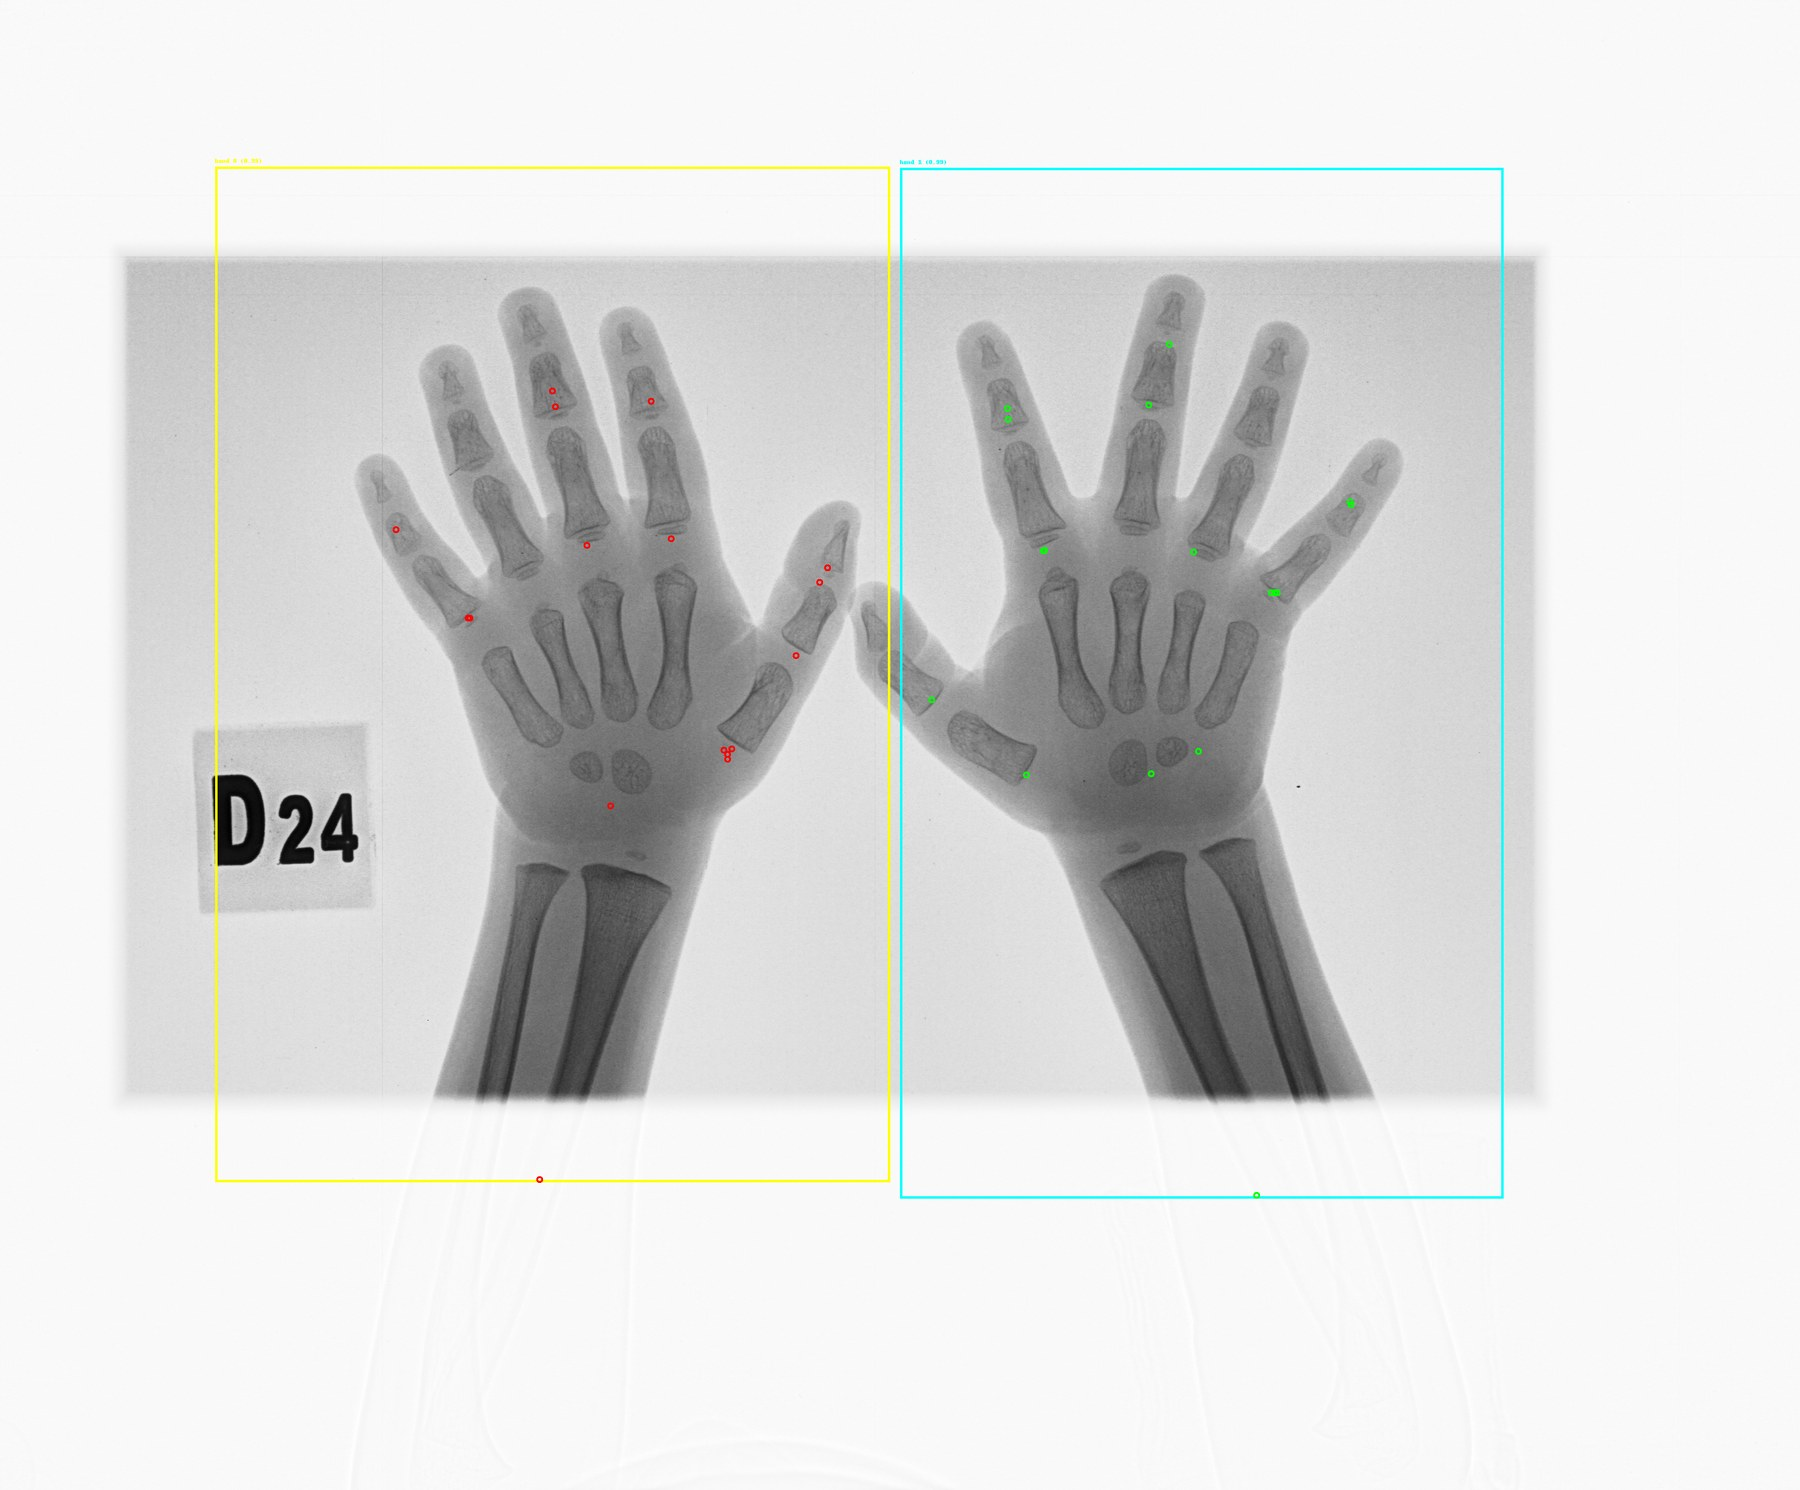
\includegraphics[width=0.48\textwidth]{figure/rhkpv3_2.jpg}
\caption{v3: immagine divisa a metà, detection e keypoint entrambi con
\texttt{mirrored}.}
\label{fig:rhkp_v3}
\end{figure}

\begin{description}
    \item[v4] Produce direttamente detection e keypoint che, a
    un'ispezione visiva, appaiono corretti per entrambe le mani, in un
    unico passaggio: a differenza di v3, qui anche i keypoint appaiono
    corretti e non solo la detection.
\end{description}

\begin{figure}[H]
\centering
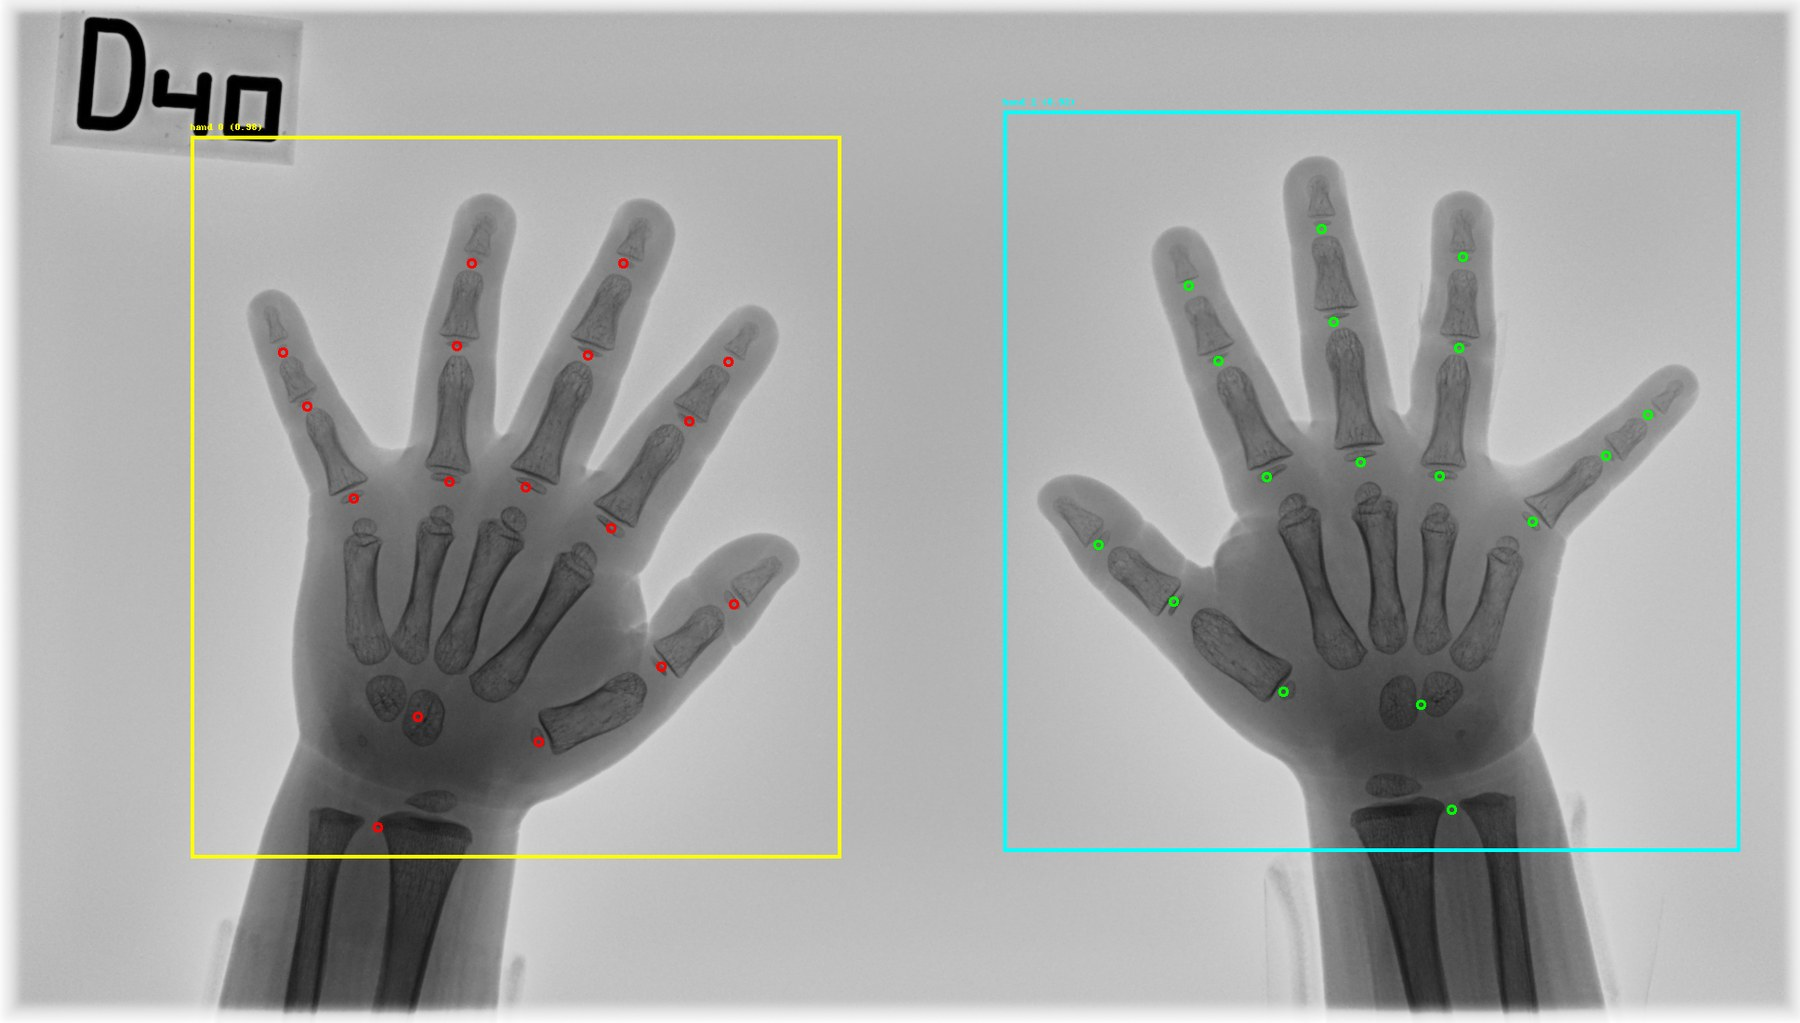
\includegraphics[width=0.48\textwidth]{figure/rhkpv4.jpg}\hfill
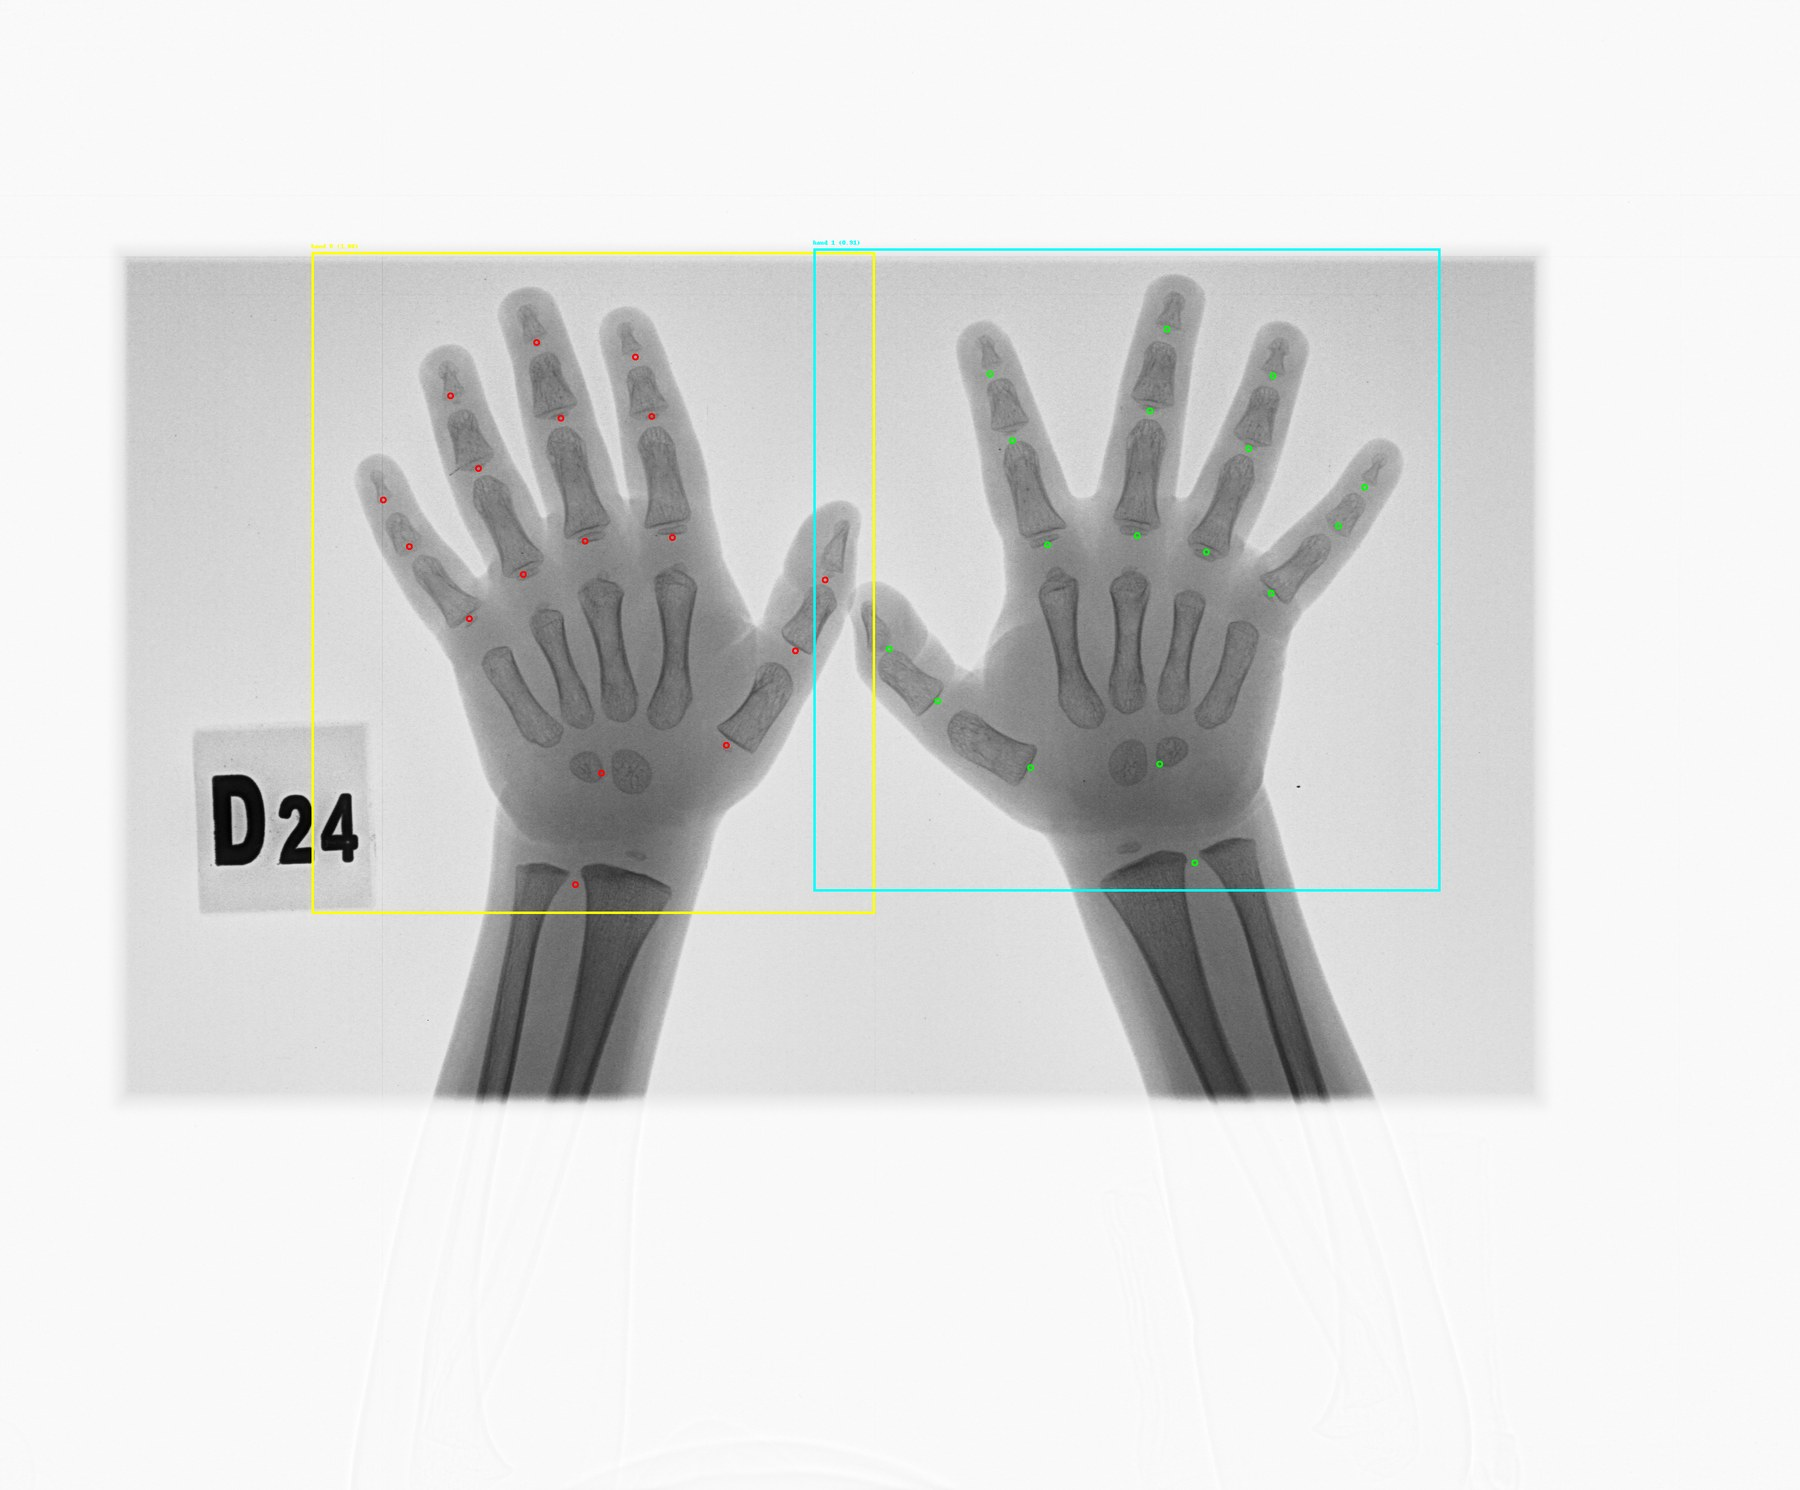
\includegraphics[width=0.48\textwidth]{figure/rhkpv4_2.jpg}
\caption{v4: singolo forward pass sull'immagine intera con
\texttt{mirrored\_full}.}
\label{fig:rhkp_v4}
\end{figure}

Tra le quattro strategie esplorate, v4 appare la più efficace ed è
coerente con i risultati quantitativi discussi in precedenza; viene
quindi adottata come soluzione di riferimento per l'obiettivo
esplorativo di predizione su entrambe le mani, tenendo conto che questa
valutazione resta qualitativa e basata su un campione ridotto di
immagini.
